\subsection{P1.1: Nonlinear regression}
Appendix A shows the code used for this assignment. The different set to be used as training, validation and test set were obtained using the built-in command \textit{randperm}. The command was used to generate a random set of numbers from 1 to the size of the dataset. Those become the indices of the numbers to create the final data set. Figure \ref{final_2_1} shows the surface of the training set.
\begin{figure}[!htbp]
\caption{Surface of training set with 1000 elements}
\label{final_2_1}
\medbreak
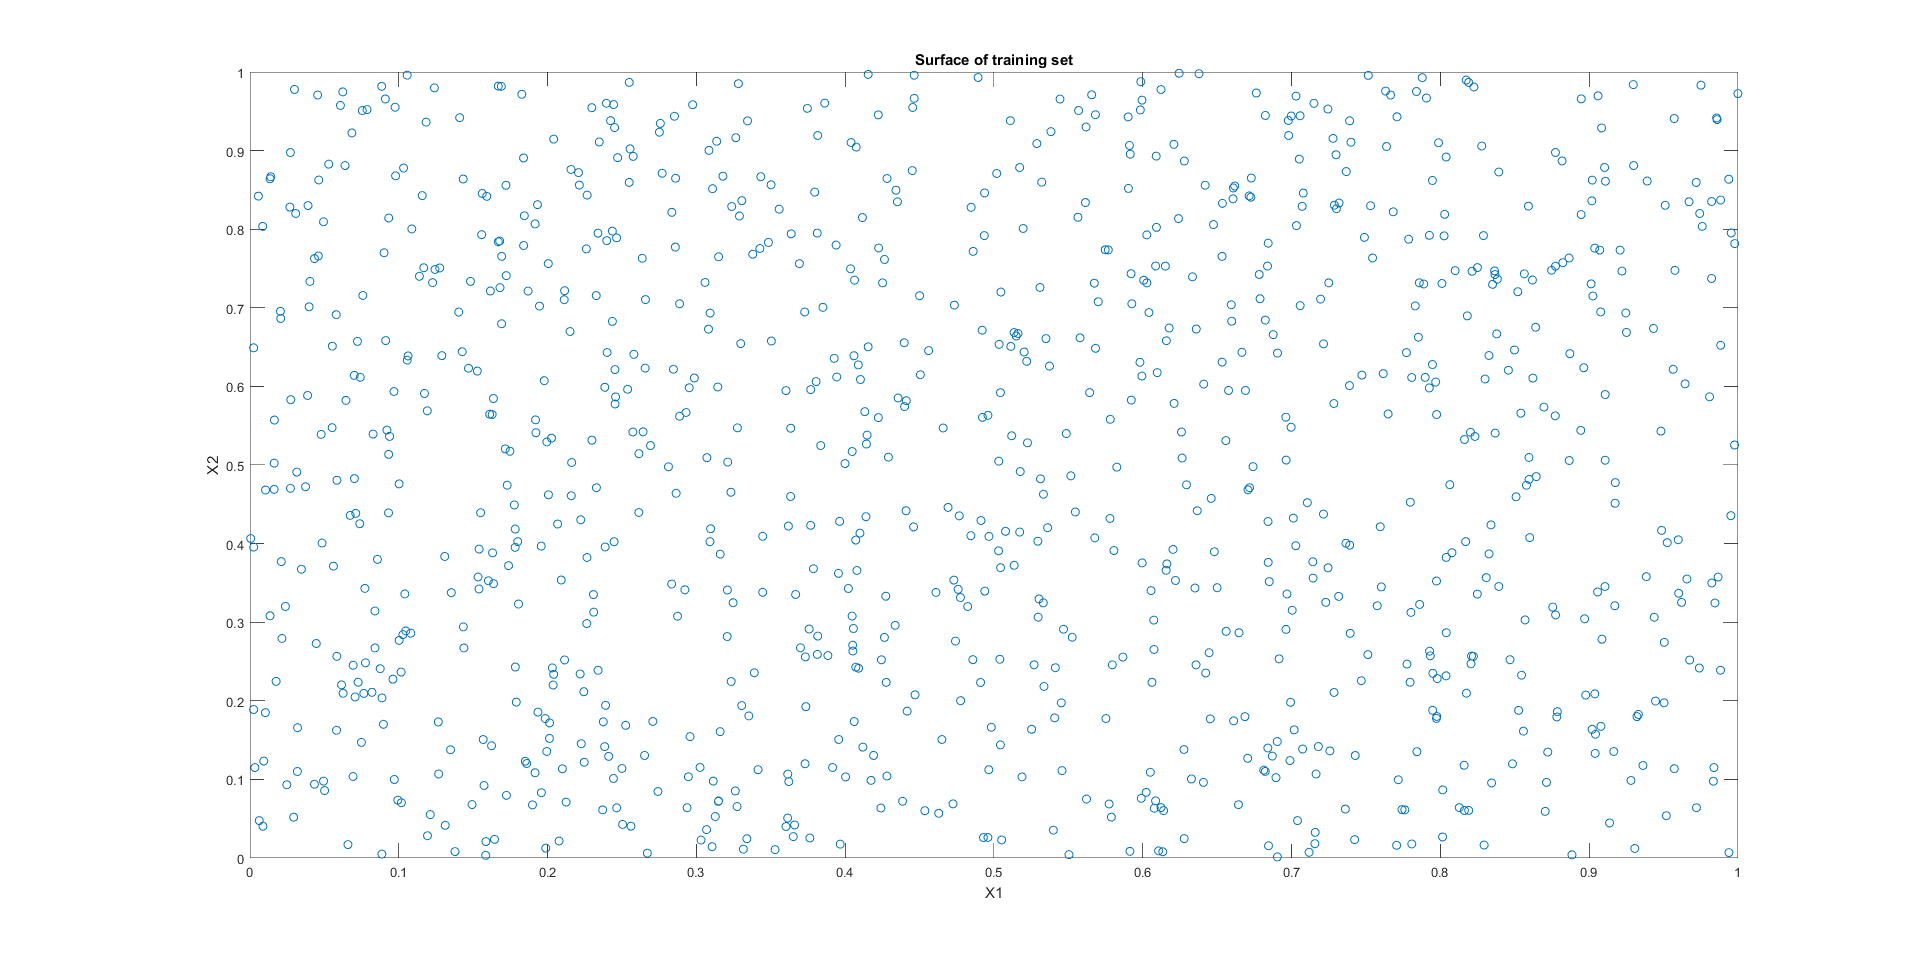
\includegraphics[width=\textwidth/3]{final/training_set_surface}
\centering
\end{figure}
\bigbreak
Based on results obtained in sections \textbf{S1} and \textbf{S4}. It was chosen to use a FFNN with one hidden layer, \textit{tansig} and \textit{purelin} as transfer functions and \textit{trainlm} as a learning algorithm. The default parameters according with \cite{matlab_2}. In order to chose a suitable number of neurons in the hidden layer, different networks were tested. According with the results in figure \ref{final_2_2}, the best model was the FFNN with 30 neurons in the hidden layer.

\begin{figure}[!htbp]
\caption{Plots of FFNN performances with different number of neurons.}
\label{final_2_2}
\medbreak
\begin{tabular}{ccc}
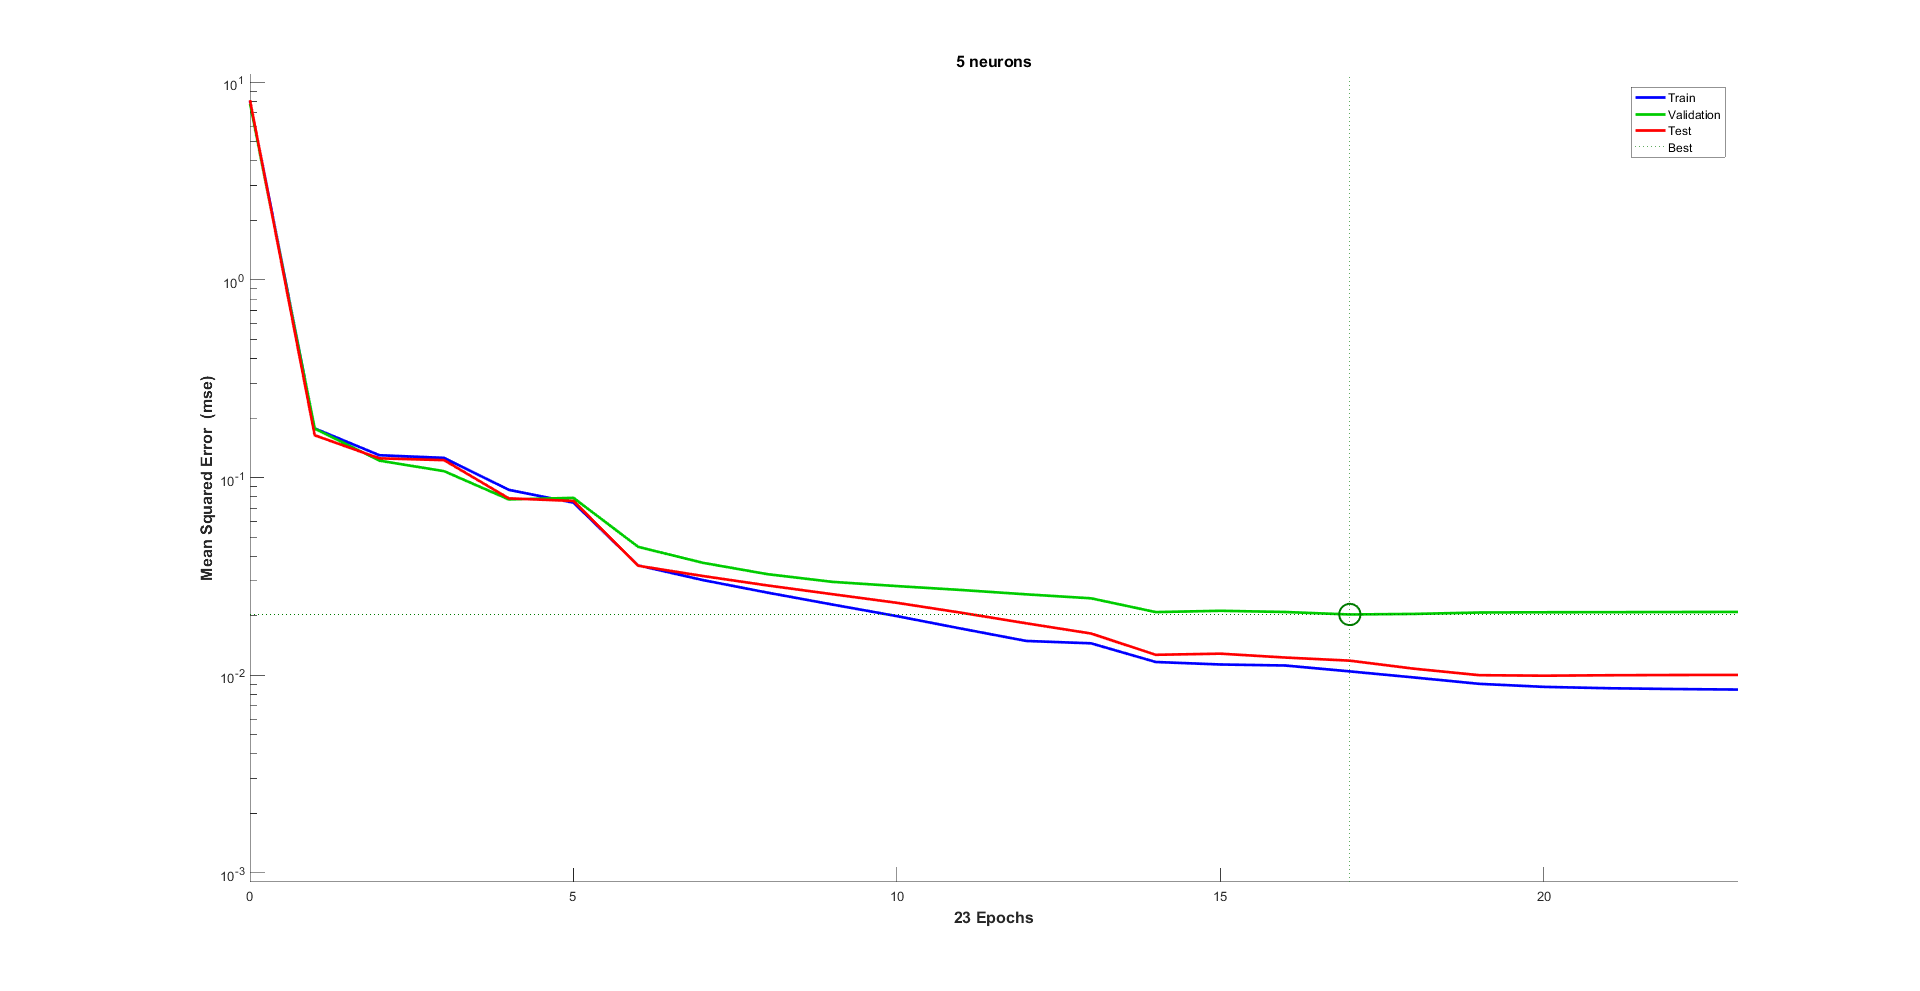
\includegraphics[width=\textwidth/4]{final/5n} &
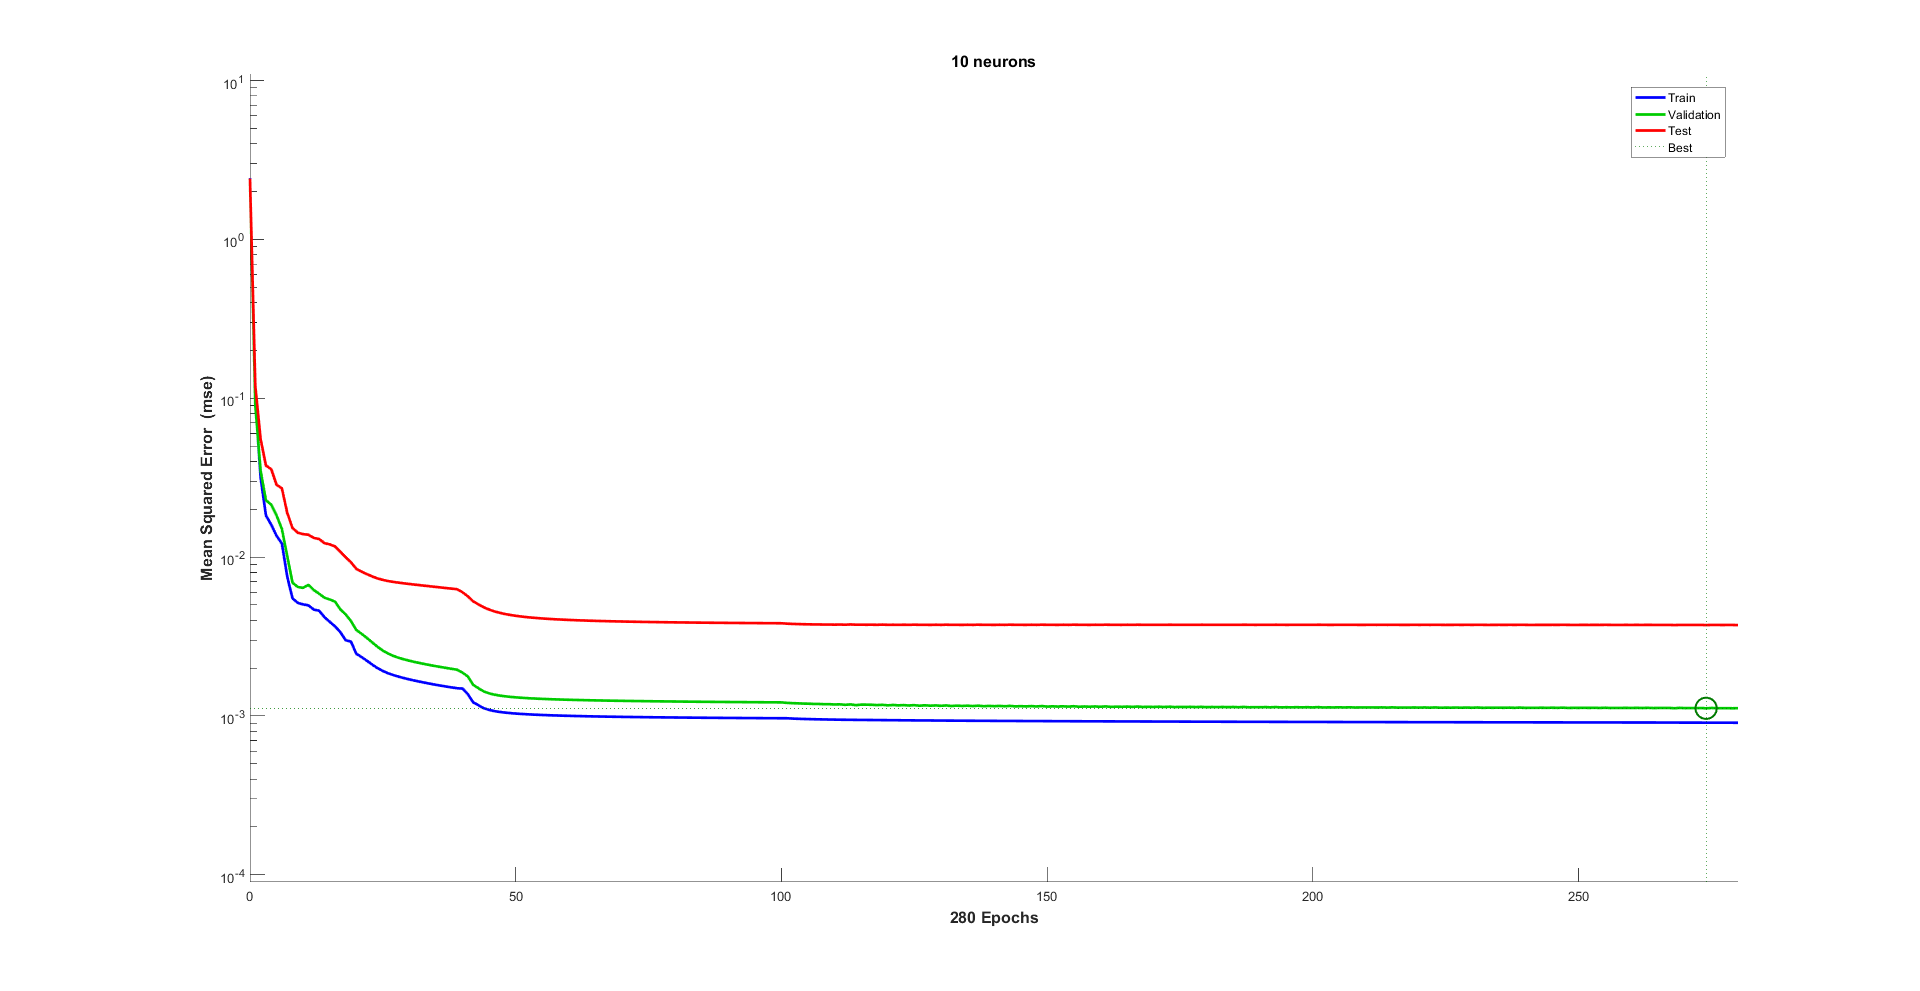
\includegraphics[width=\textwidth/4]{final/10n} &
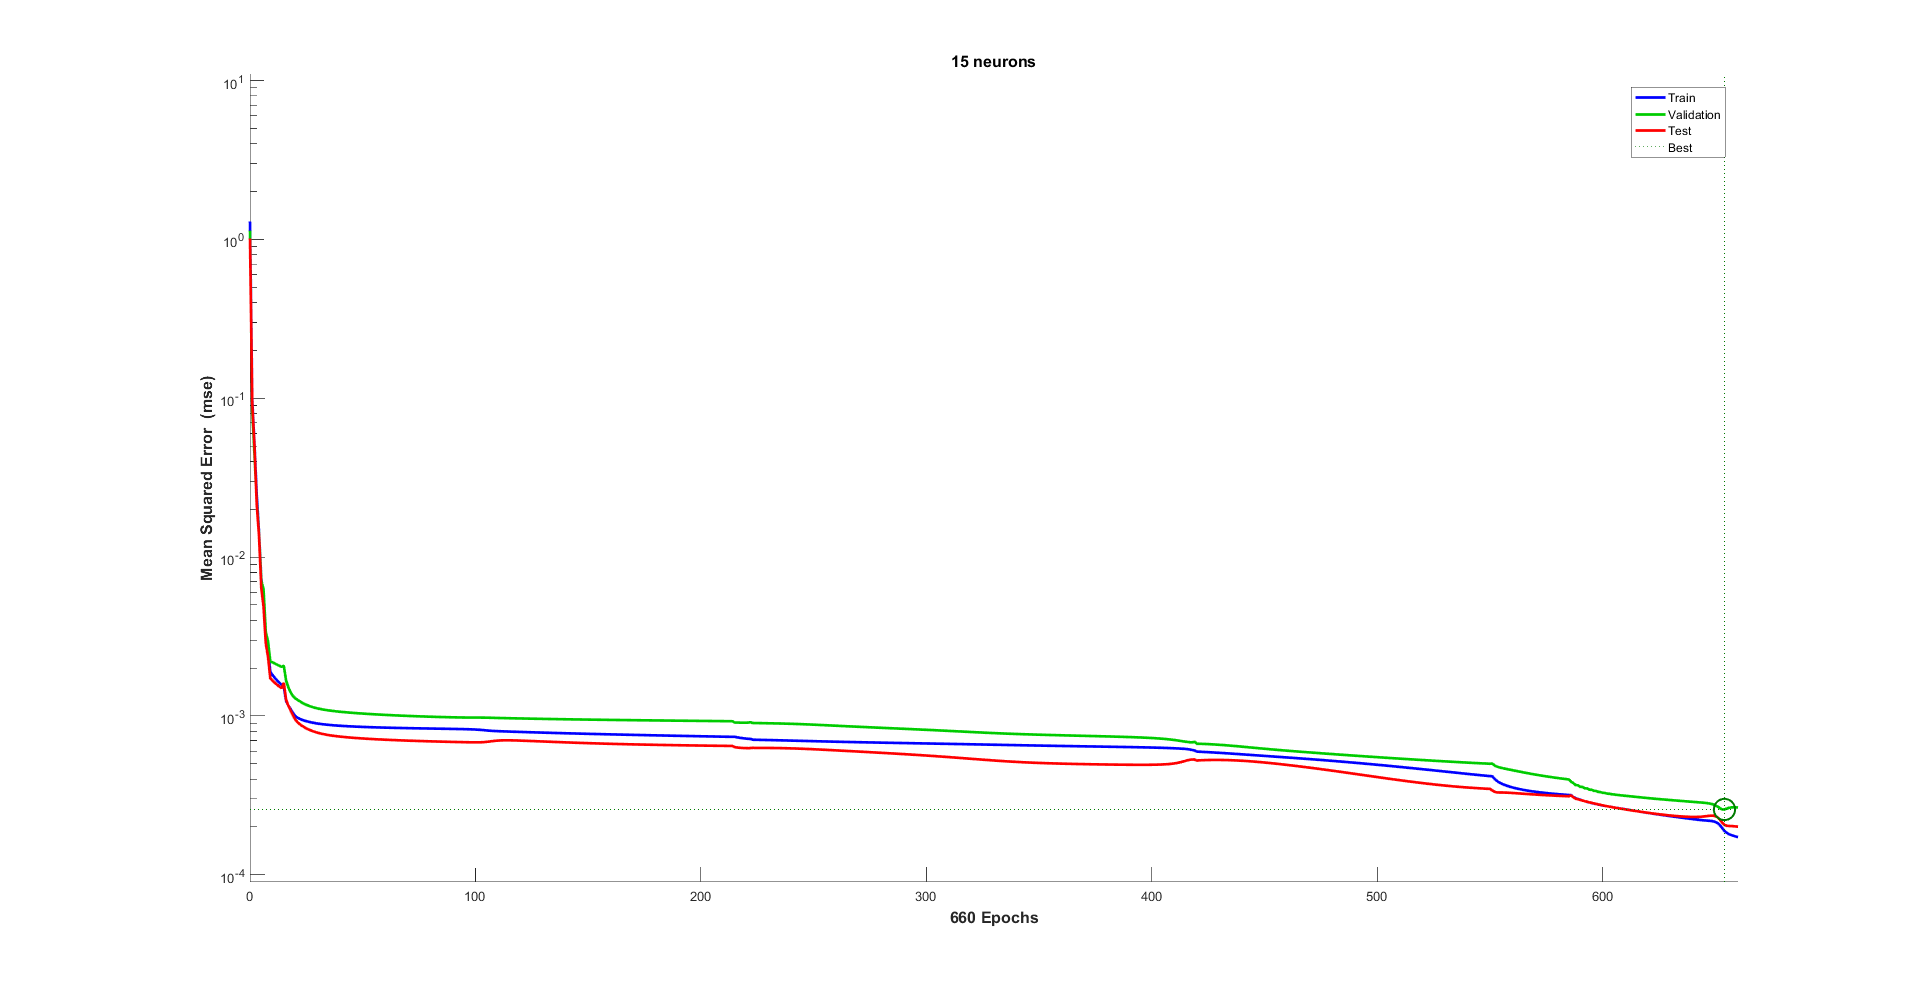
\includegraphics[width=\textwidth/4]{final/15n} \\
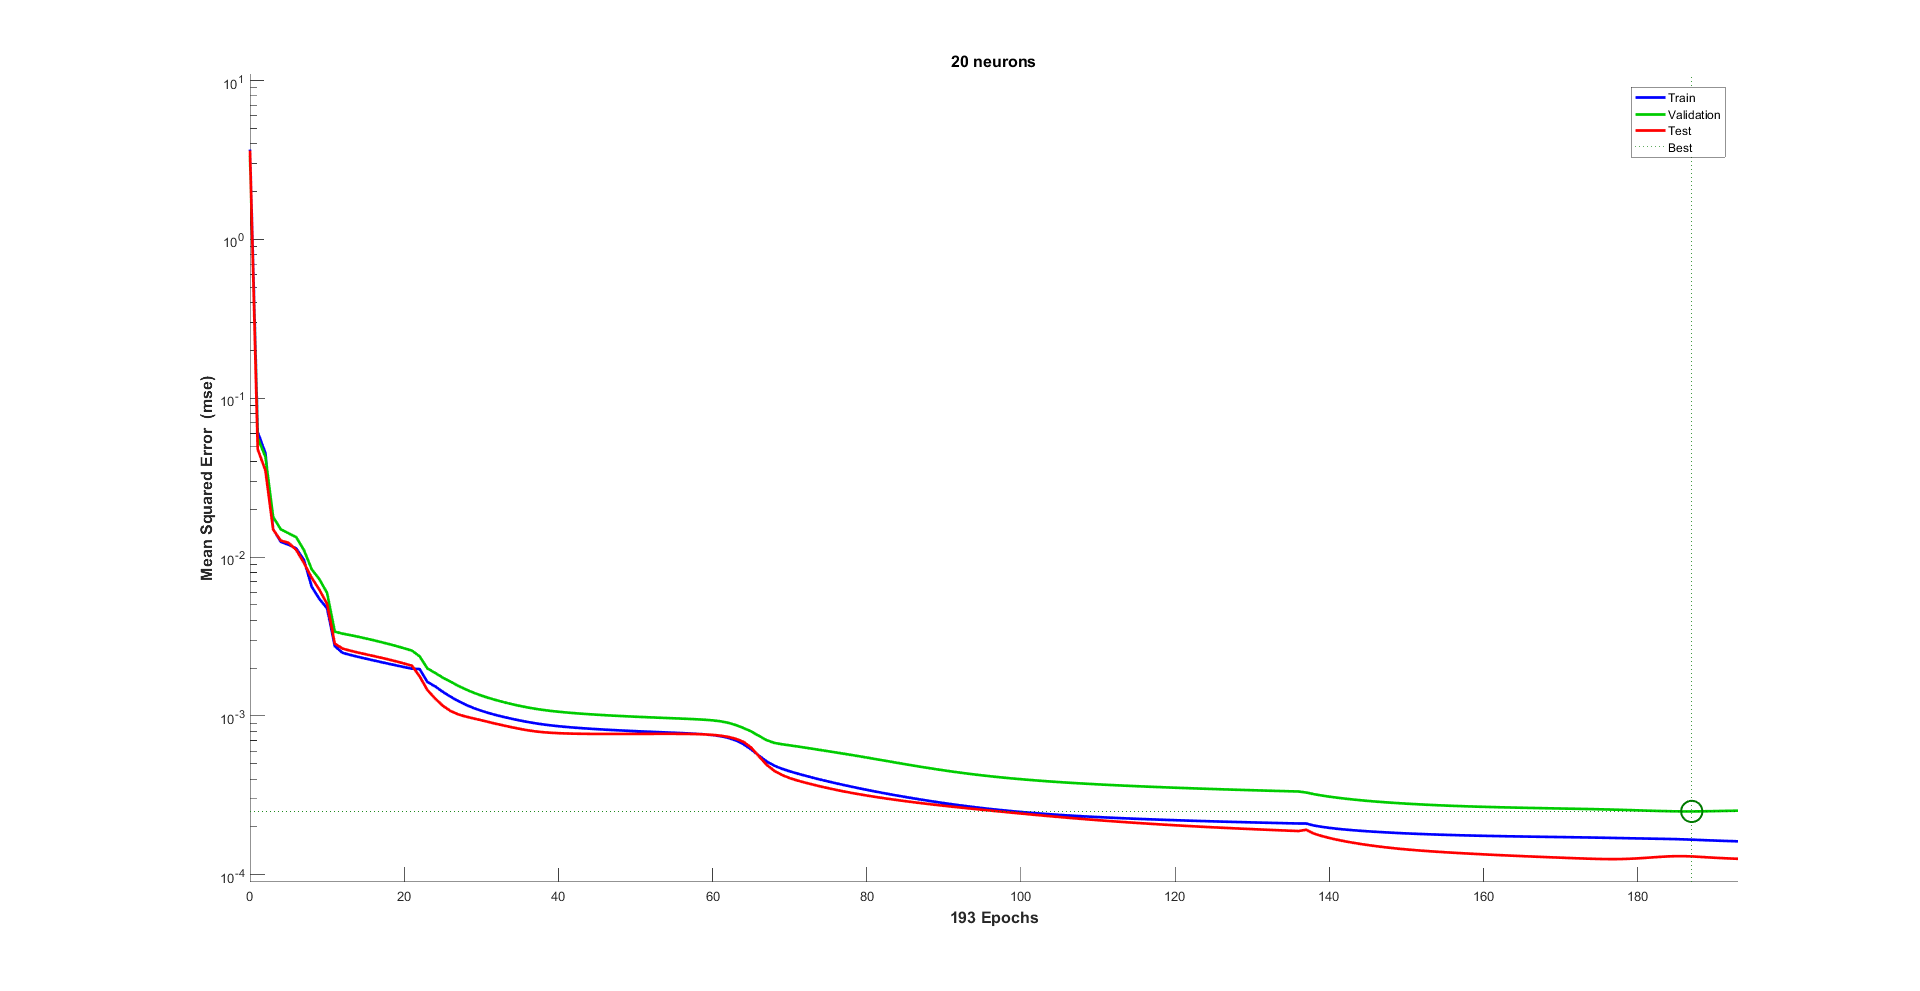
\includegraphics[width=\textwidth/4]{final/20n} &
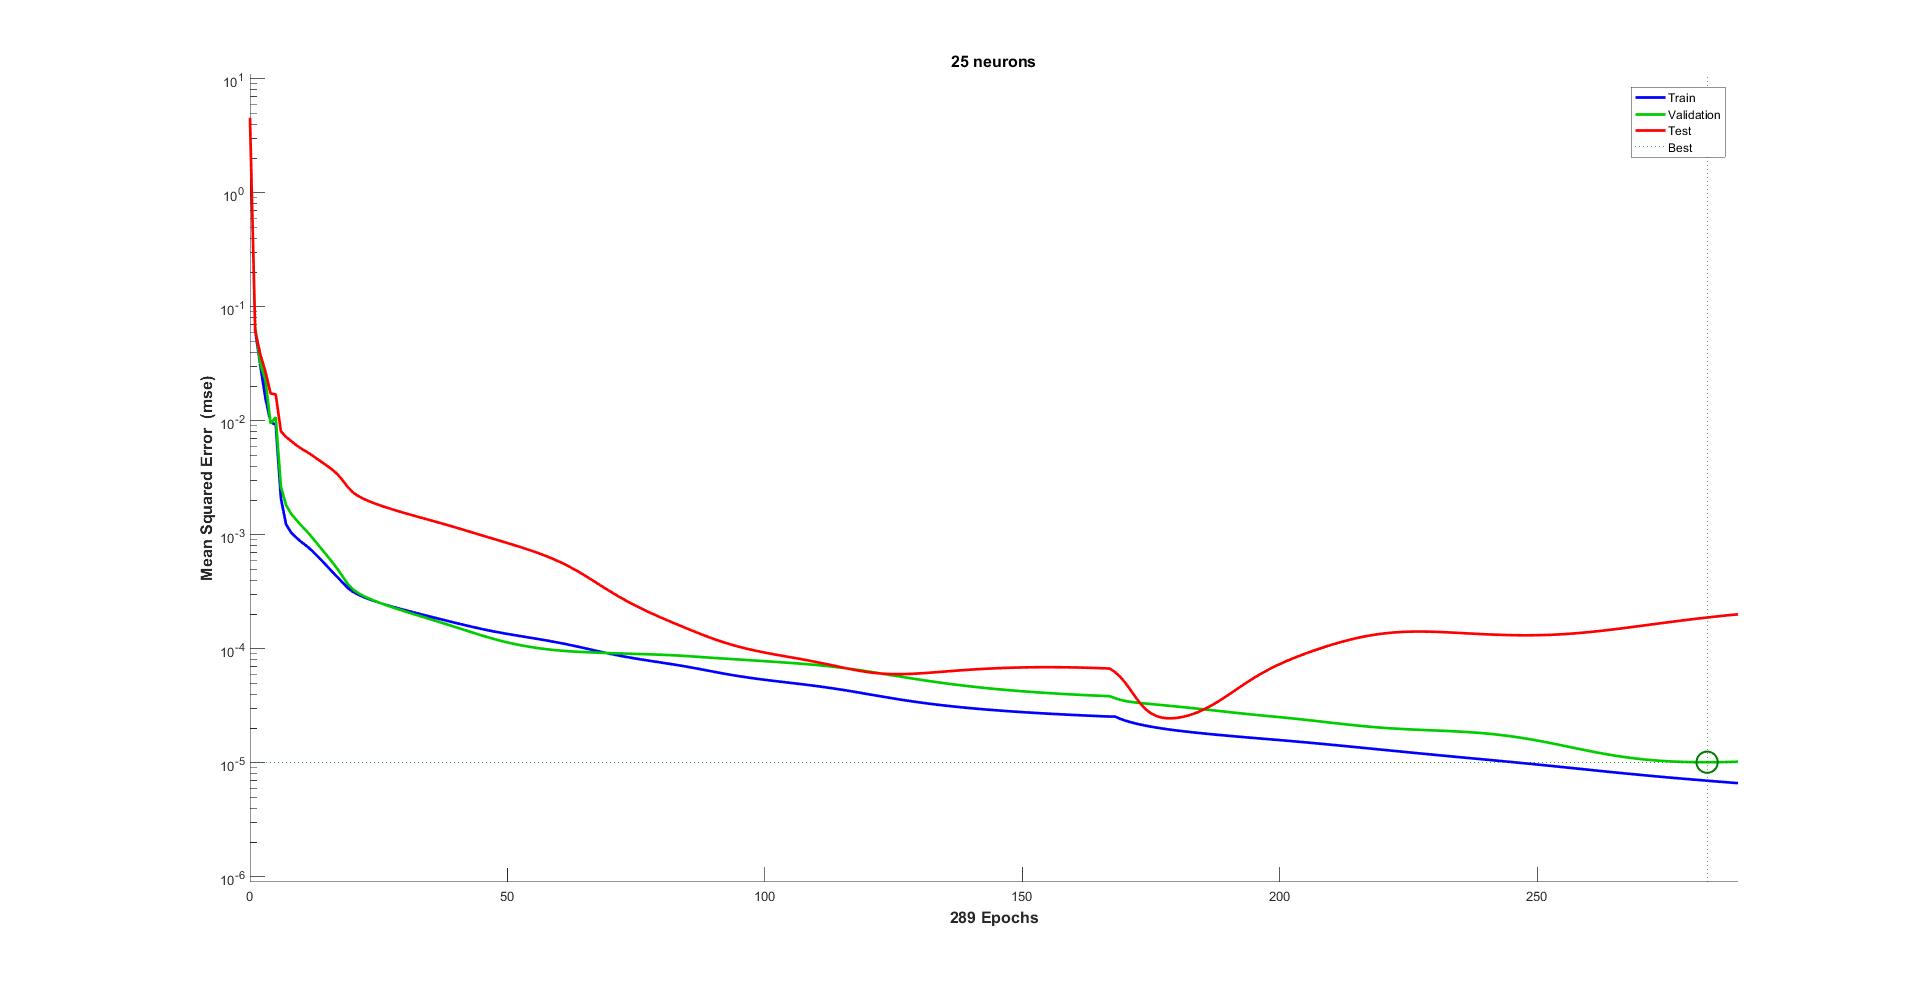
\includegraphics[width=\textwidth/4]{final/25n} &
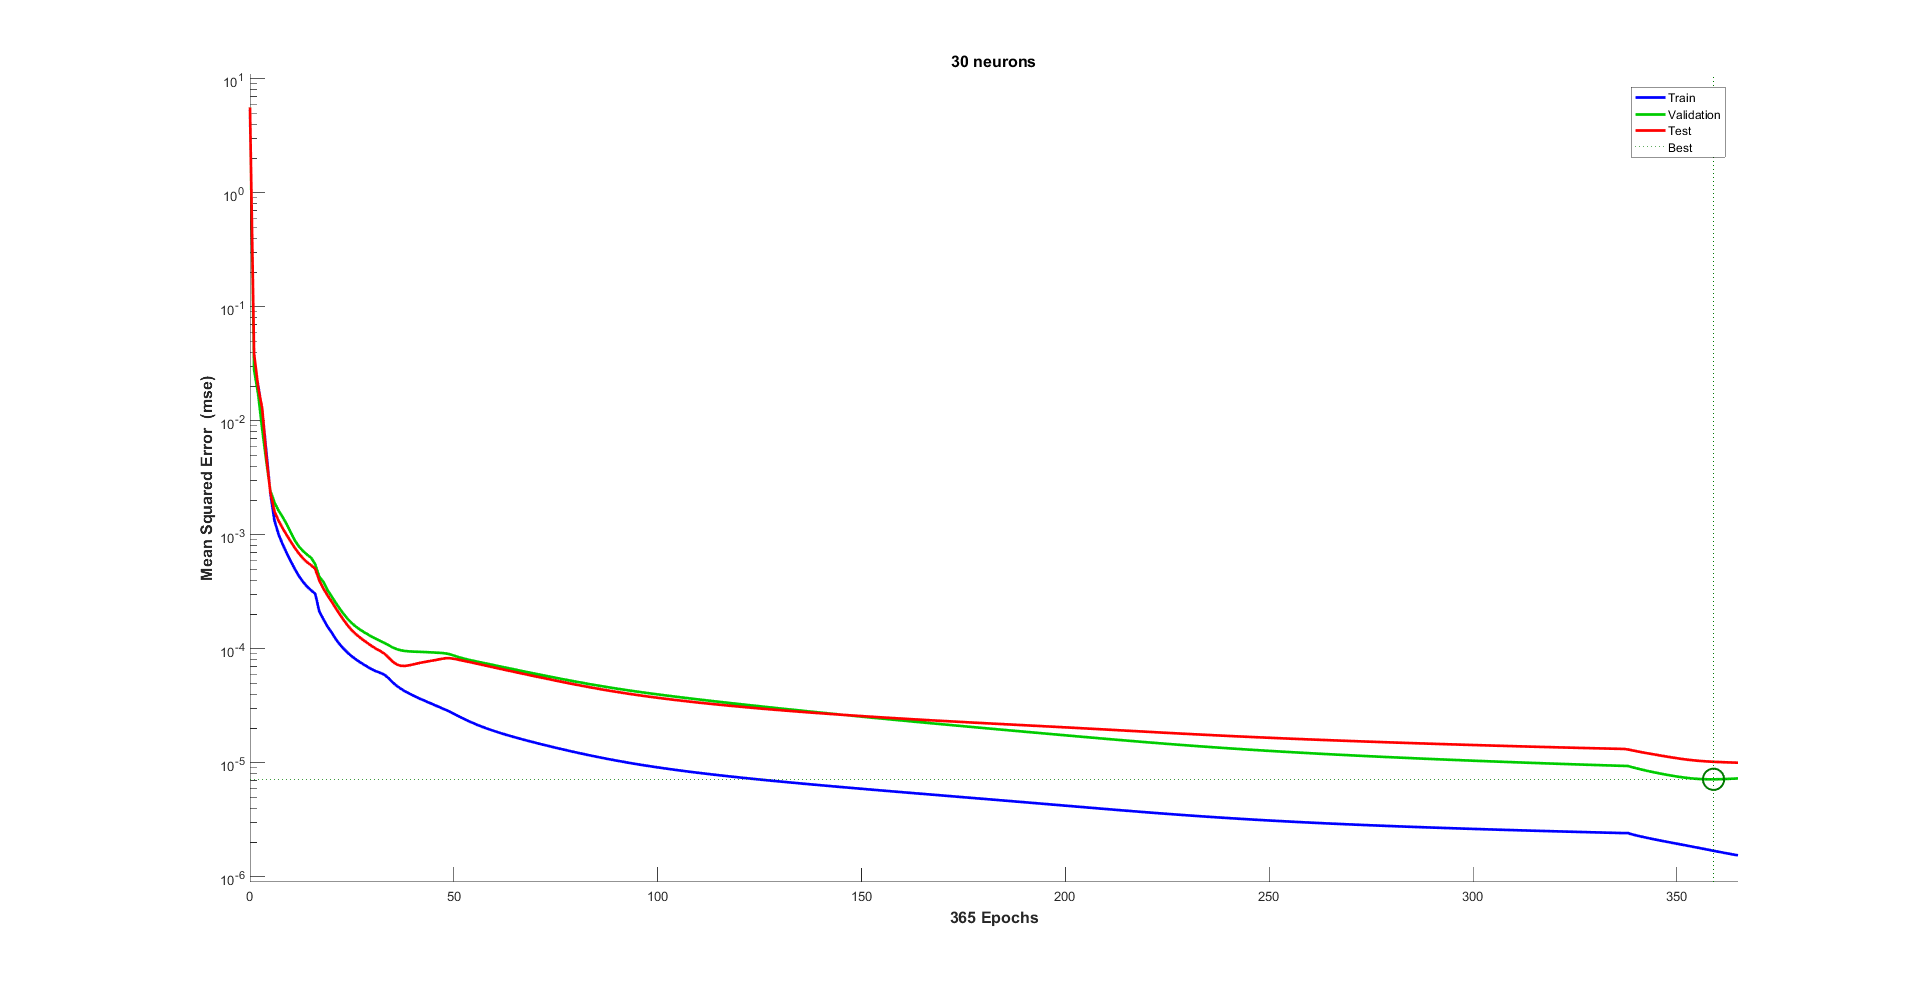
\includegraphics[width=\textwidth/4]{final/30n}
\end{tabular}
\centering
\end{figure}

Finally the performance of the chosen model was assessed using the test set. A total of 100 iterations using different random seeds were run in order to avoid naive results. The MSE average of the model was 1.1736e-05. Figure \ref{final_2_3} shows the result of one of the iterations, in this case the MSE was 1.6656e-06.

\begin{figure}[!htbp]
\caption{Plot of the ground truth (blue surface) and prediction surface (red surface).}
\label{final_2_3}
\medbreak
\begin{tabular}{ccc}
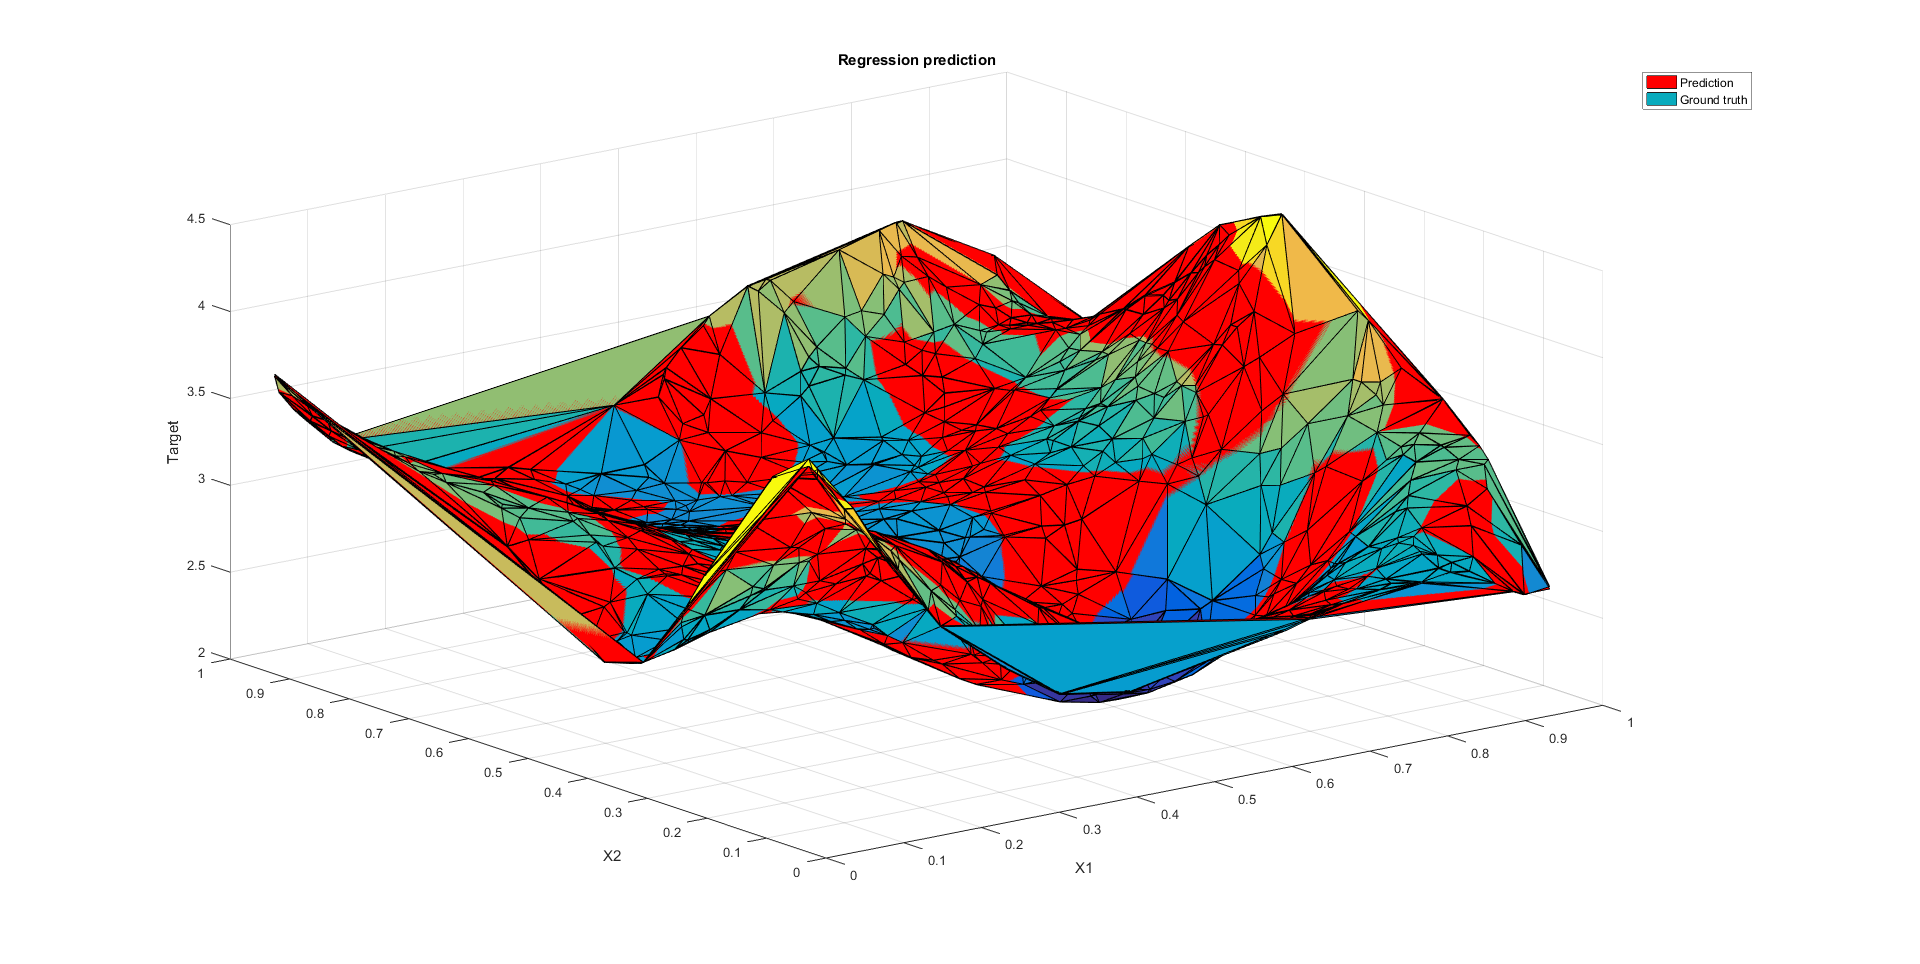
\includegraphics[width=\textwidth/4]{final/test_prediction_surface1} &
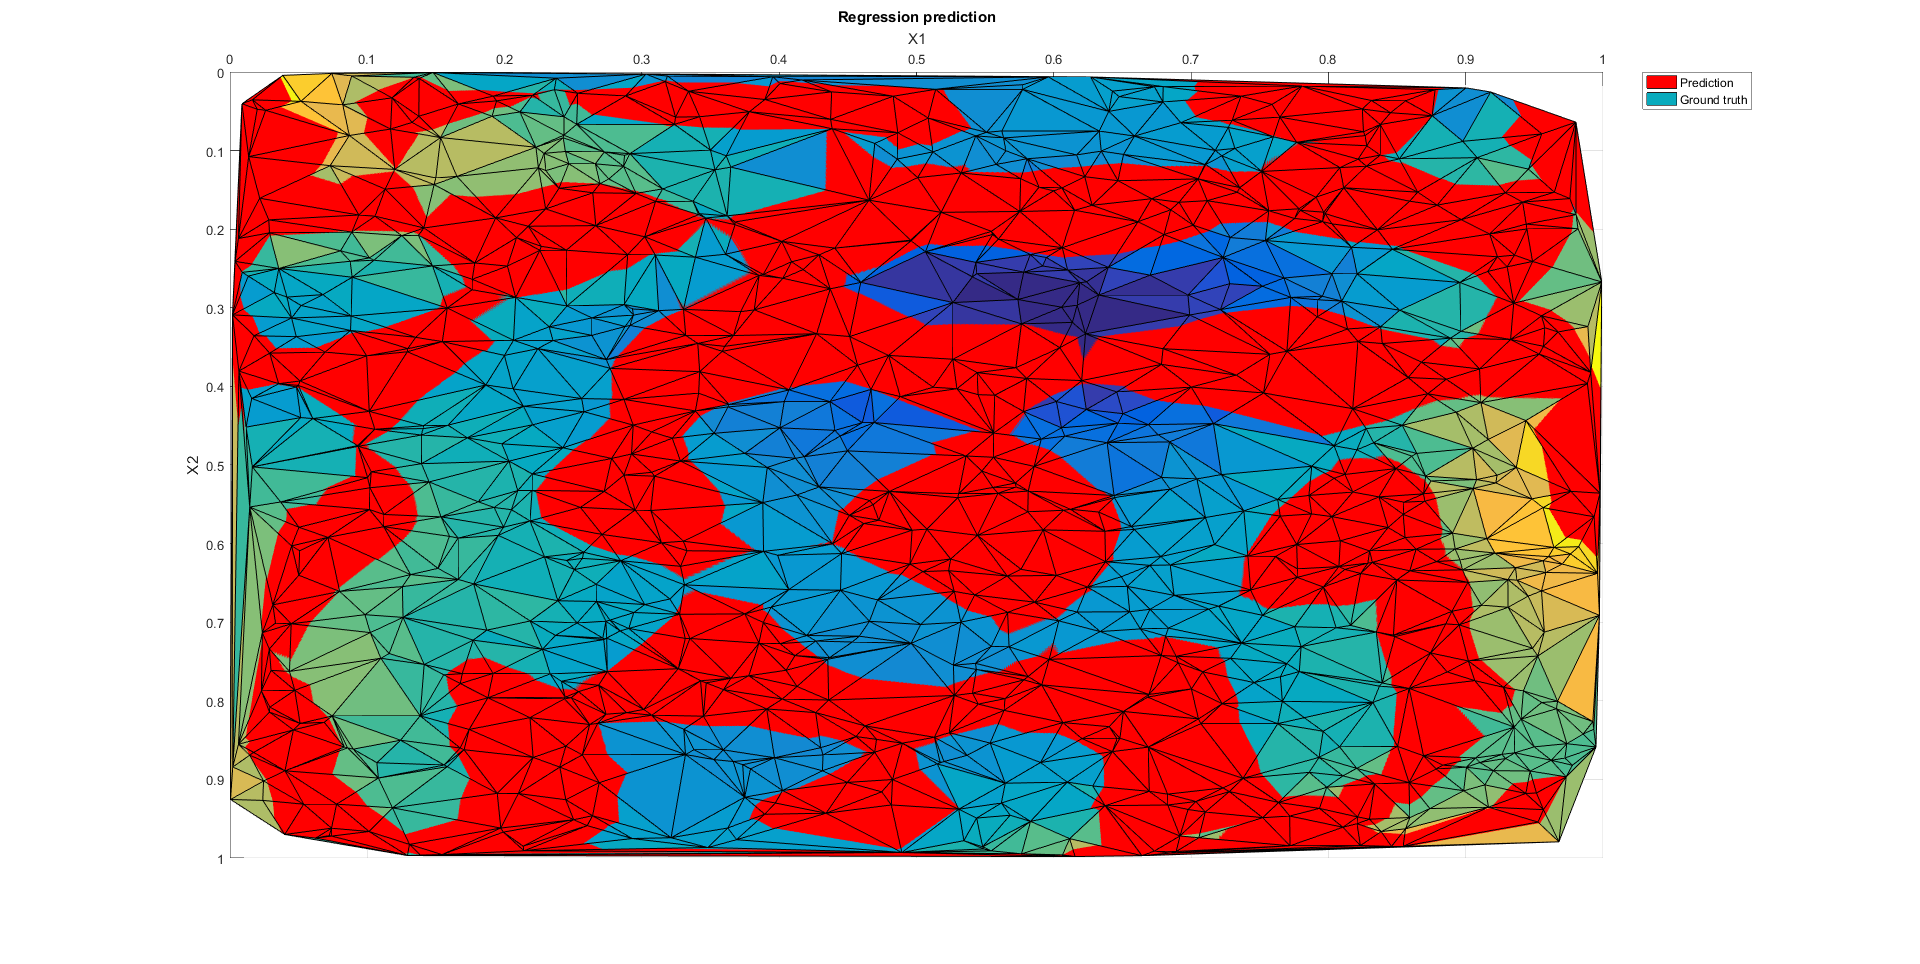
\includegraphics[width=\textwidth/4]{final/test_prediction_surface2} &
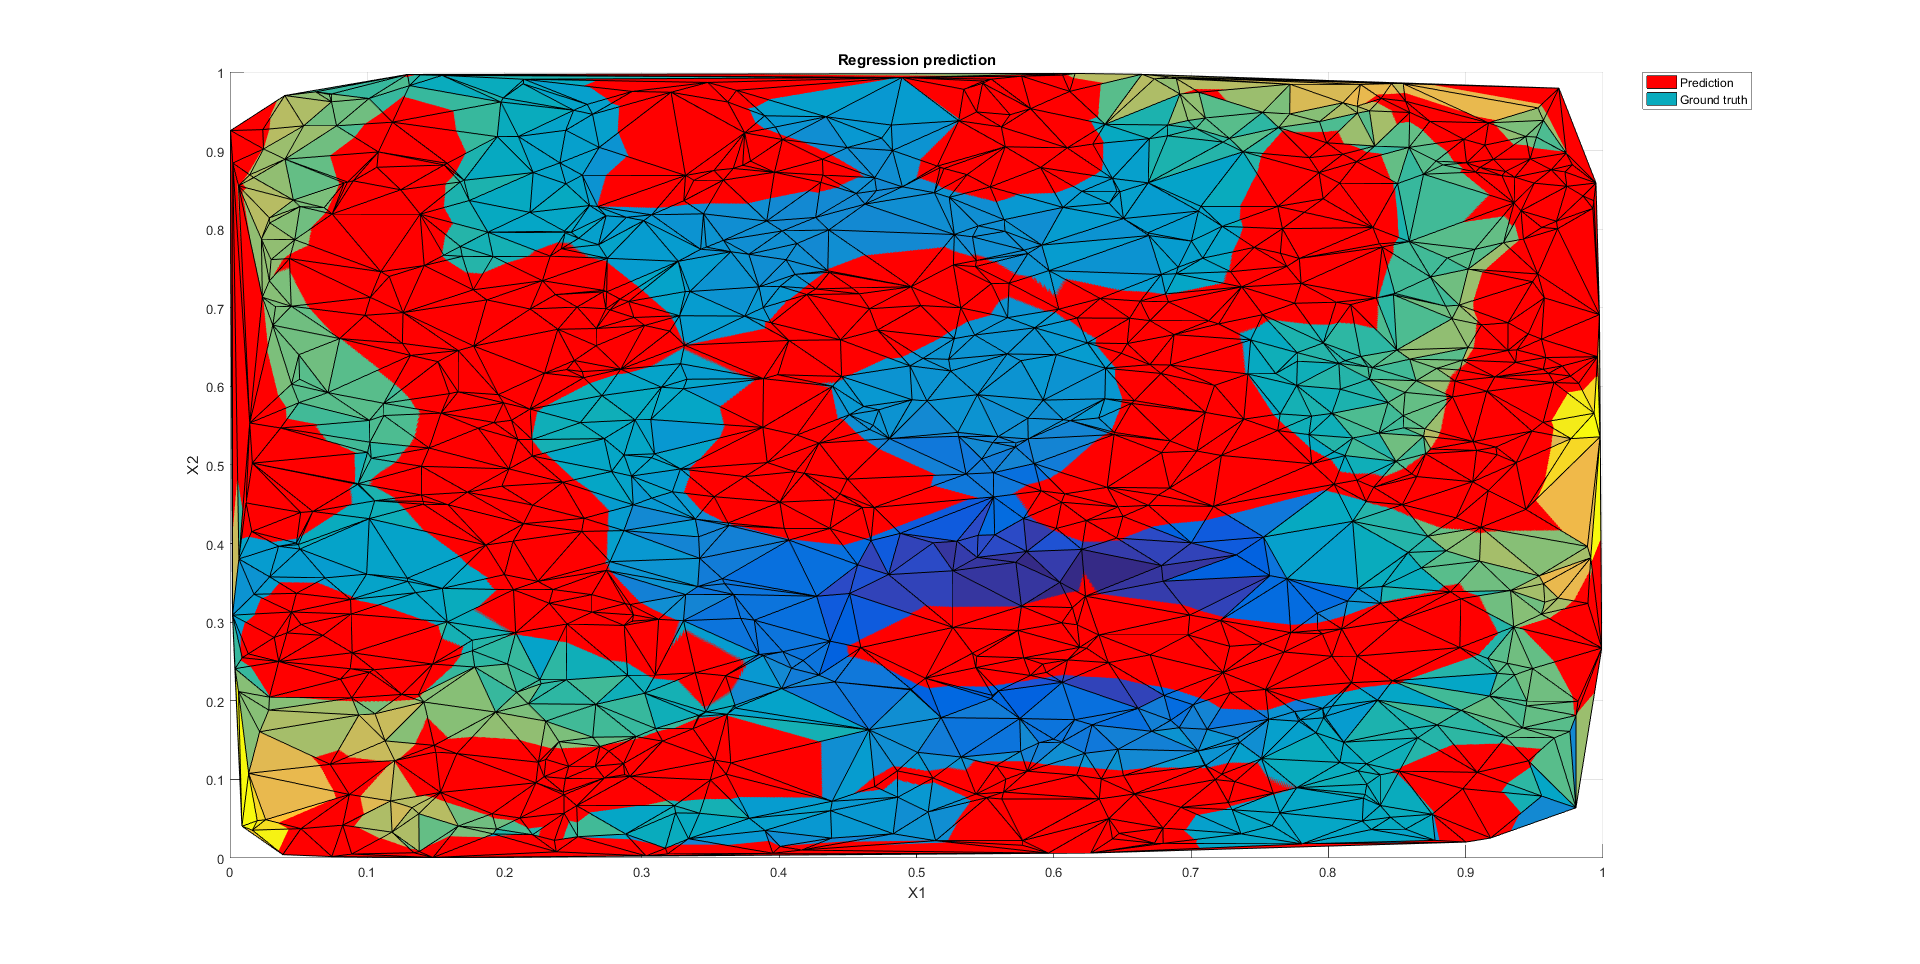
\includegraphics[width=\textwidth/4]{final/test_prediction_surface3}
\end{tabular}
\centering
\end{figure}

\subsection{P1.2: Classification}
The same FFNN architecture, as previous section, was used. Different number of neurons were test in order to set best. Figure \ref{final_3__01} shows the results of the test. According with the results and in contrast with the previous section, the best number of neurons for this specific tasks was 45.

\begin{figure}[!htbp]
\caption{Results of the classification tasks using different number of neurons}
\label{final_3__01}
\medbreak
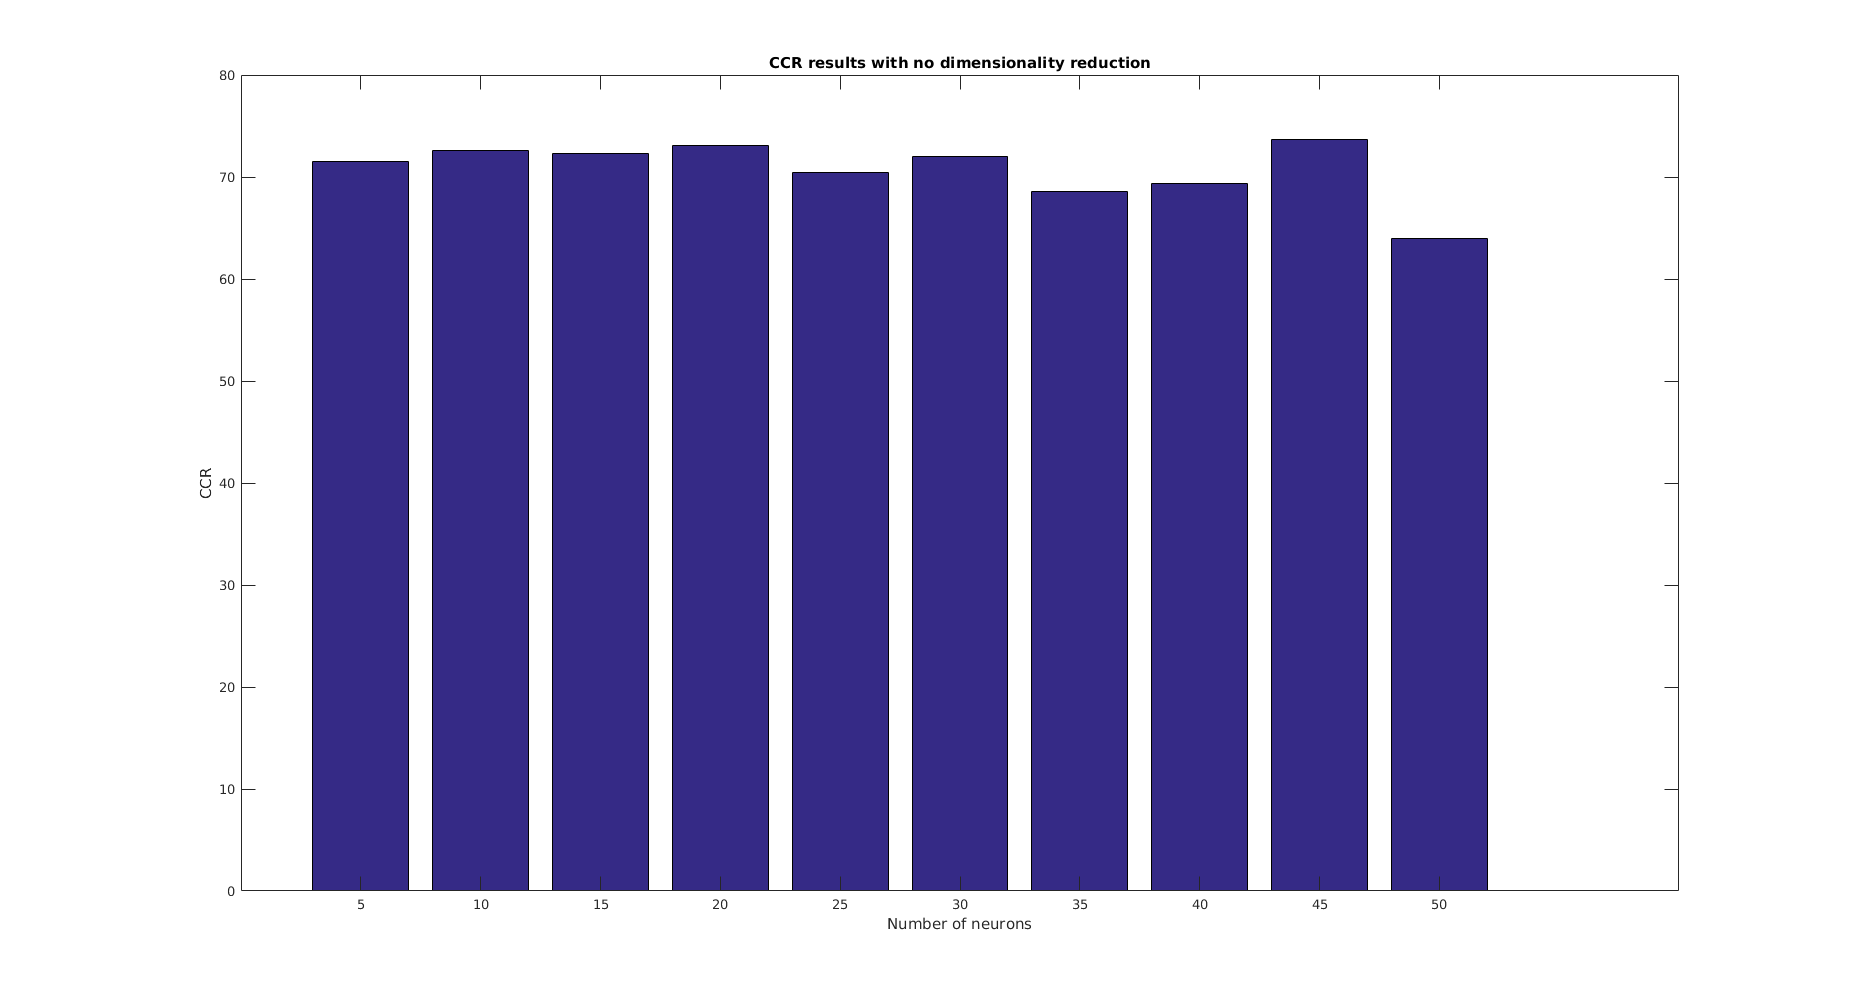
\includegraphics[width=\textwidth/3]{final/preset_fnn_no_dimensionality_reduction}
\centering
\end{figure}

The PCA algorithm was implemented using the code of section \textbf{S3}. Different k componentes were test. Using the knowledge obtained from the experiments of section \textbf{S3} and the results of figure \ref{final_3_2fff}, it was deduced that the best k was 3. In figure \ref{final_3_2fff}, one can see that there is a decay of the cumulative largest values after the third component, which state that after it, there error of the reconstruction will not be reduced dramatically.

\begin{figure}[!htbp]
\caption{Results of the classification tasks using different number of neurons}
\label{final_3_2fff}
\medbreak
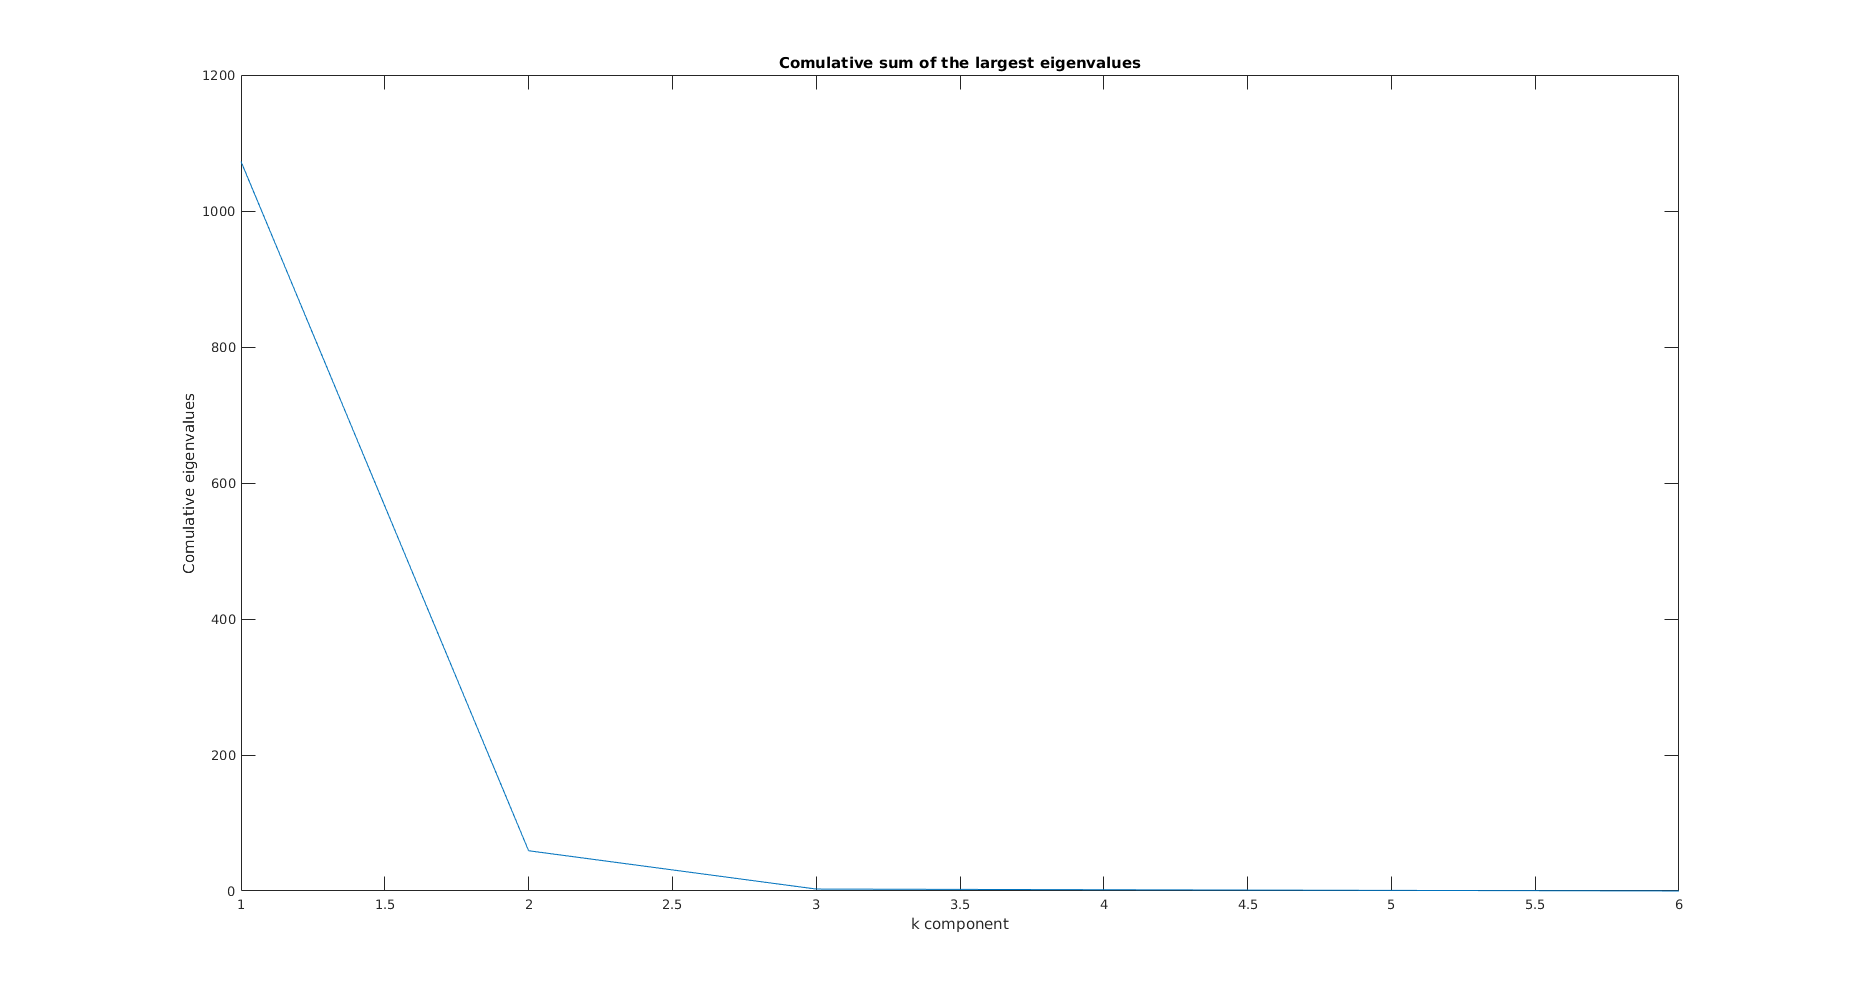
\includegraphics[width=\textwidth/3]{final/comulative_eigenvalues}
\centering
\end{figure}

A final experiment was set, know using the lower dimension data set. In order to have big picture of the different k values and different FFNN models, all the combinations were run. Figure \ref{final_3_3} shows the results. It was noticed that k=3, although it was showed as a good value for PCA, was not necessary the best value. k between 5 and 6 performs better, depending on the number of neurons in the hidden layer.

\begin{figure}[!htbp]
\caption{Results of the classification tasks using different number of neurons}
\label{final_3_3}
\medbreak
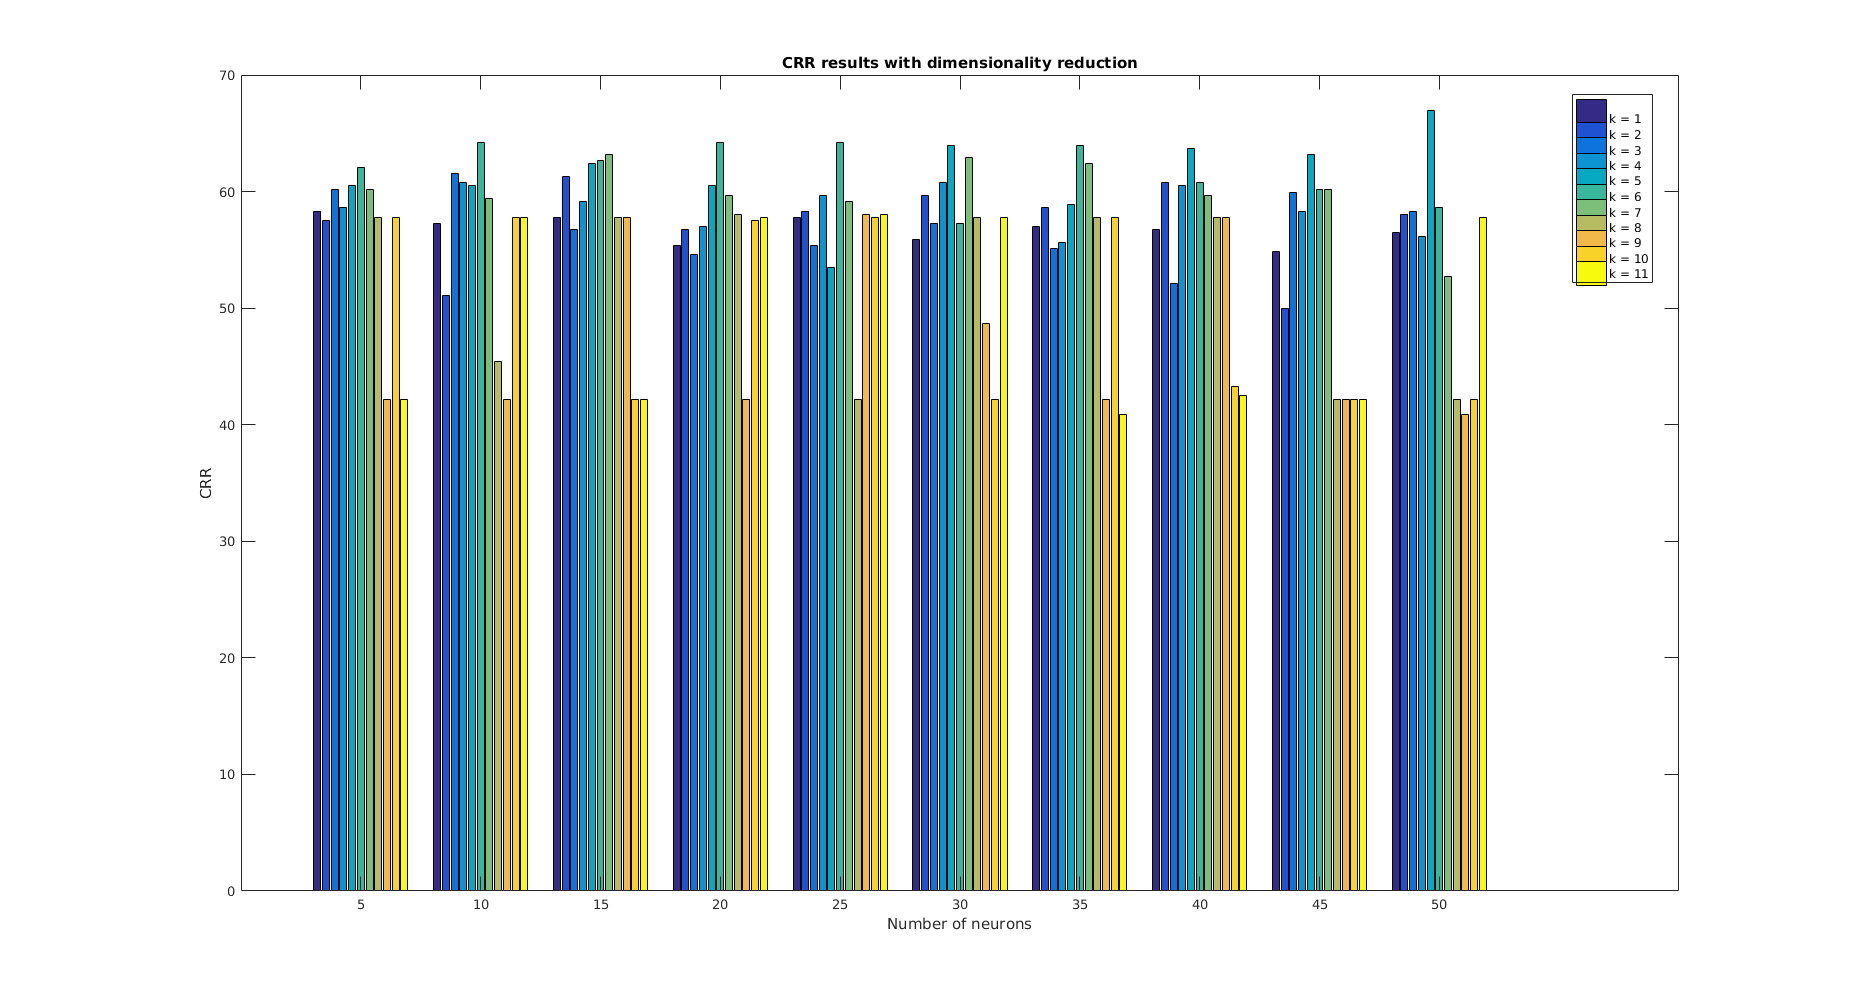
\includegraphics[width=\textwidth/3]{final/preset_fnn_reduction}
\centering
\end{figure}

Additionally, the overall performance is lower, which indicates that the dataset is sensible to dimensionality reduction. It is reasonable since the dimension is not as big as the dimension of the data set used in section \textbf{S3}. Besides, the the dataset might be high correlated which decreased the performance of the PCA algorithm which can imply a reduction of the performance of the FFNN. It is concluded that inputs are as important as the model of the neural networks; the better the quality of the inputs (features) are, the better the performance of the neural network is. 

\subsection{P2: Character recognition with Hopfield networks}
As warm-up task, the required letters were created and added to the vocabulary. Figure \ref{all_letter} shows the final results.

\begin{figure}[!htbp]
\caption{Set of letter in the dataset (attractors)}
\label{all_letter}
\medbreak
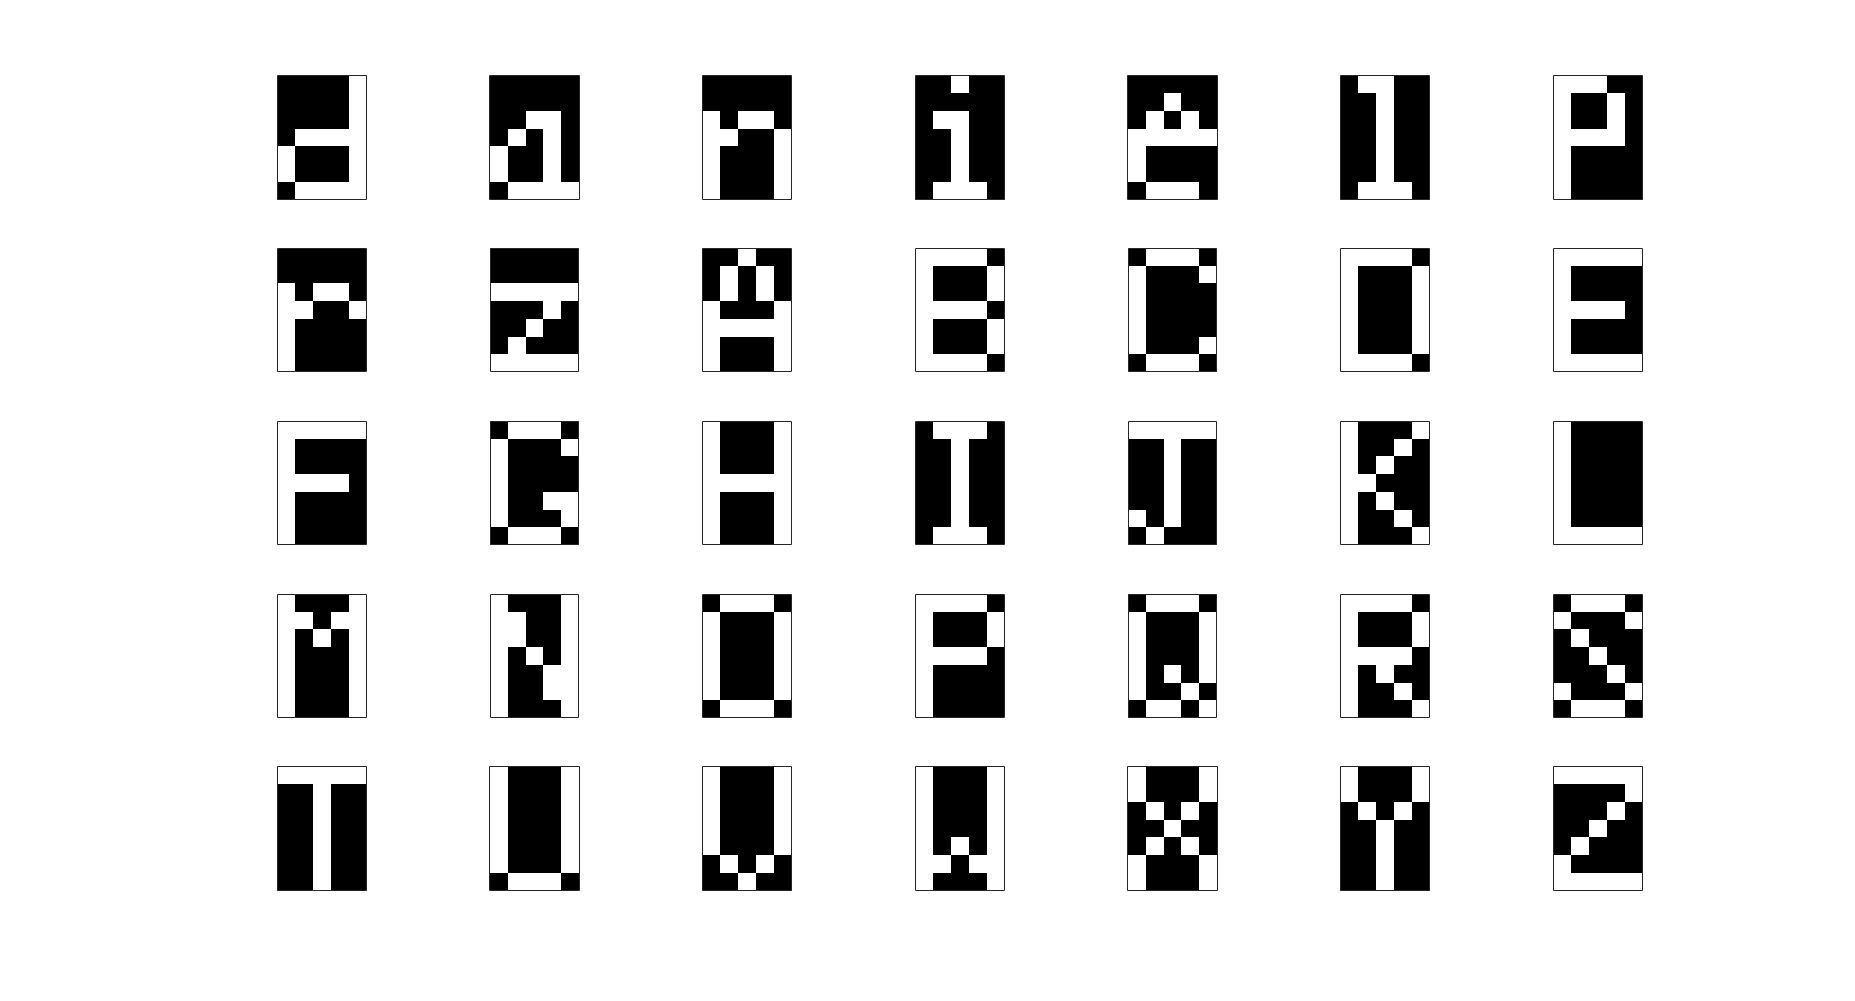
\includegraphics[width=\textwidth/2]{final/all_letters}
\centering
\end{figure}

In order to tested the accuracy of the Hopfield network, 10,000 iterations were tested using different distorted patterns. Figure \ref{final_3_1} shows the results of one of the iterations. This Hopfield network could recall perfectly the numbers, a MSE average of 0 was obtained. After an exhaustive set of tests, no spurious patterns were found. 

\begin{figure}[!htbp]
\caption{Top: original letter (attractor state). Middle: distorted letter by 3 pixeles. Bottom: reconstruction using the Hopfield network.}
\label{final_3_1}
\medbreak
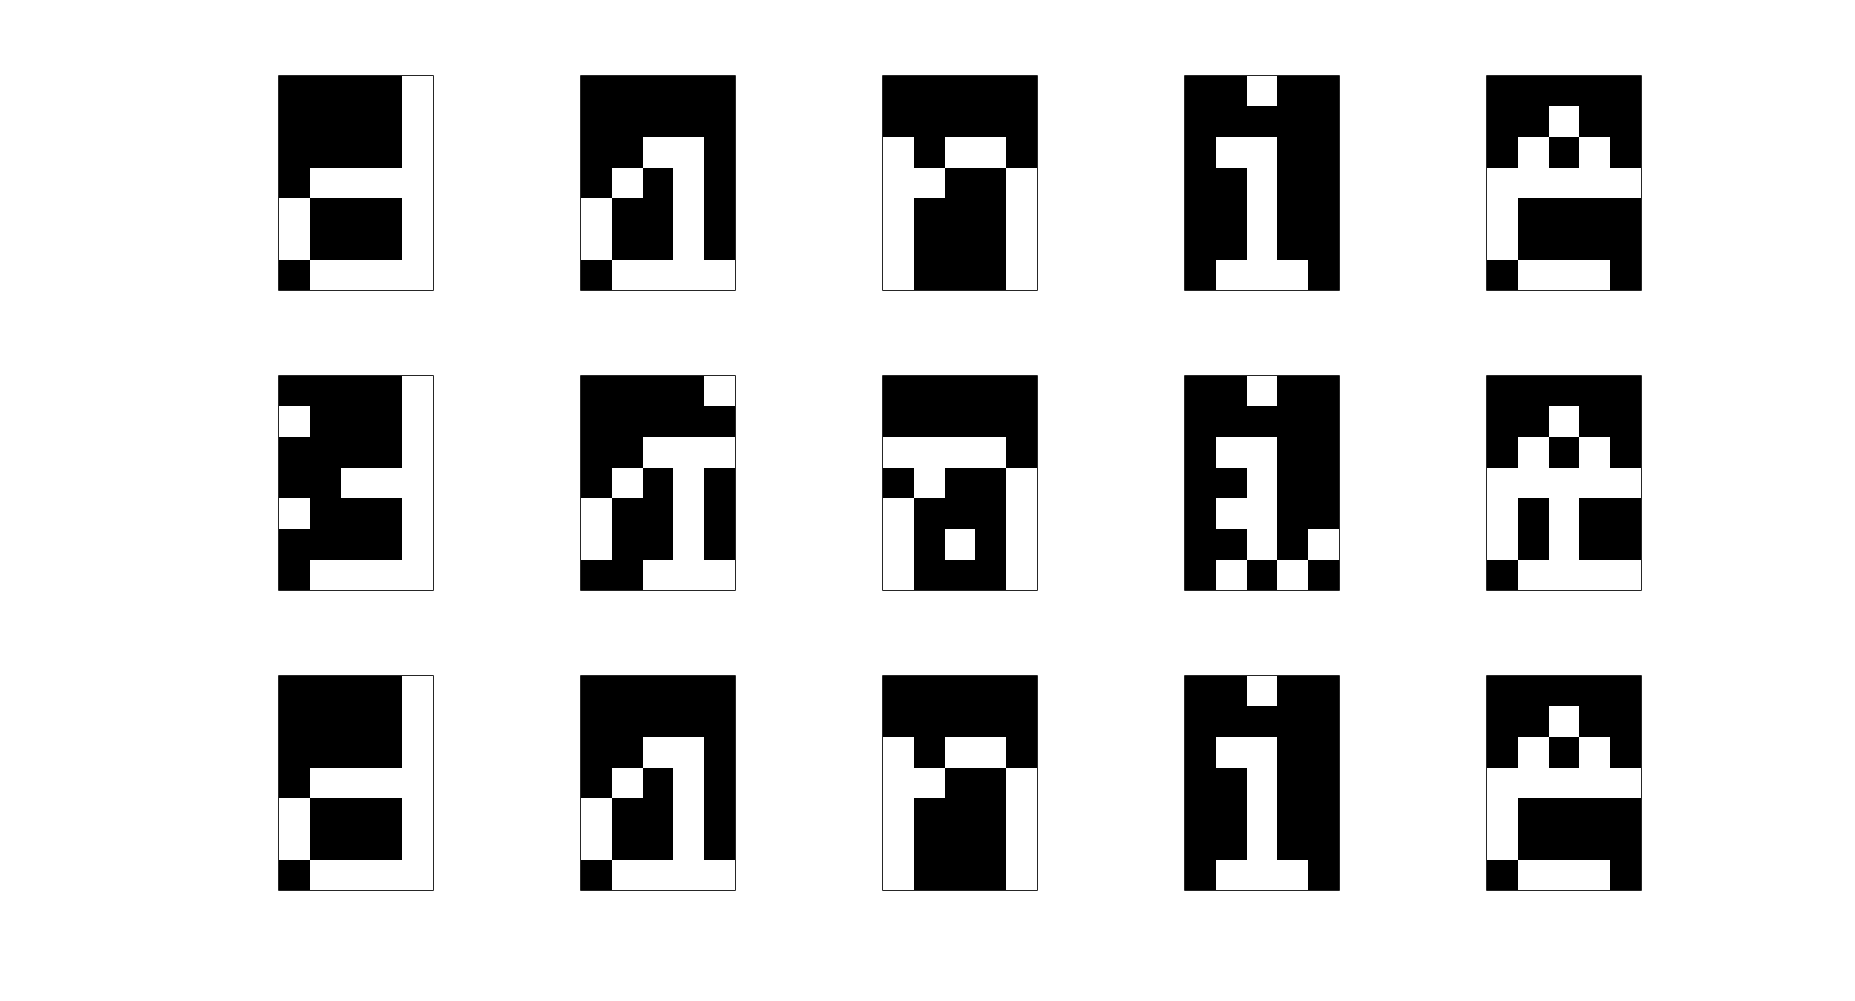
\includegraphics[width=\textwidth/2]{final/tasks_2}
\centering
\end{figure}

After the initial experiment, different values of P were tested with 100 epochs. The results of the experiments are shown in figure \ref{spurious_error_state}. This experiments show that the maximum capacity of attractors to generated a perfect recall is roughly 5. This empirical results shown that the theoretical loading capacity using the Hebb-rule (figure \ref{teoretical_hebb}) can be a little off with the actual capacity. However it is a good estimation in order to prevent unexpected states (spurious patterns).


\begin{figure}[!htbp]
\caption{Average of absolute error and number of spurious patterns found with different P values.}
\label{spurious_error_state}
\medbreak
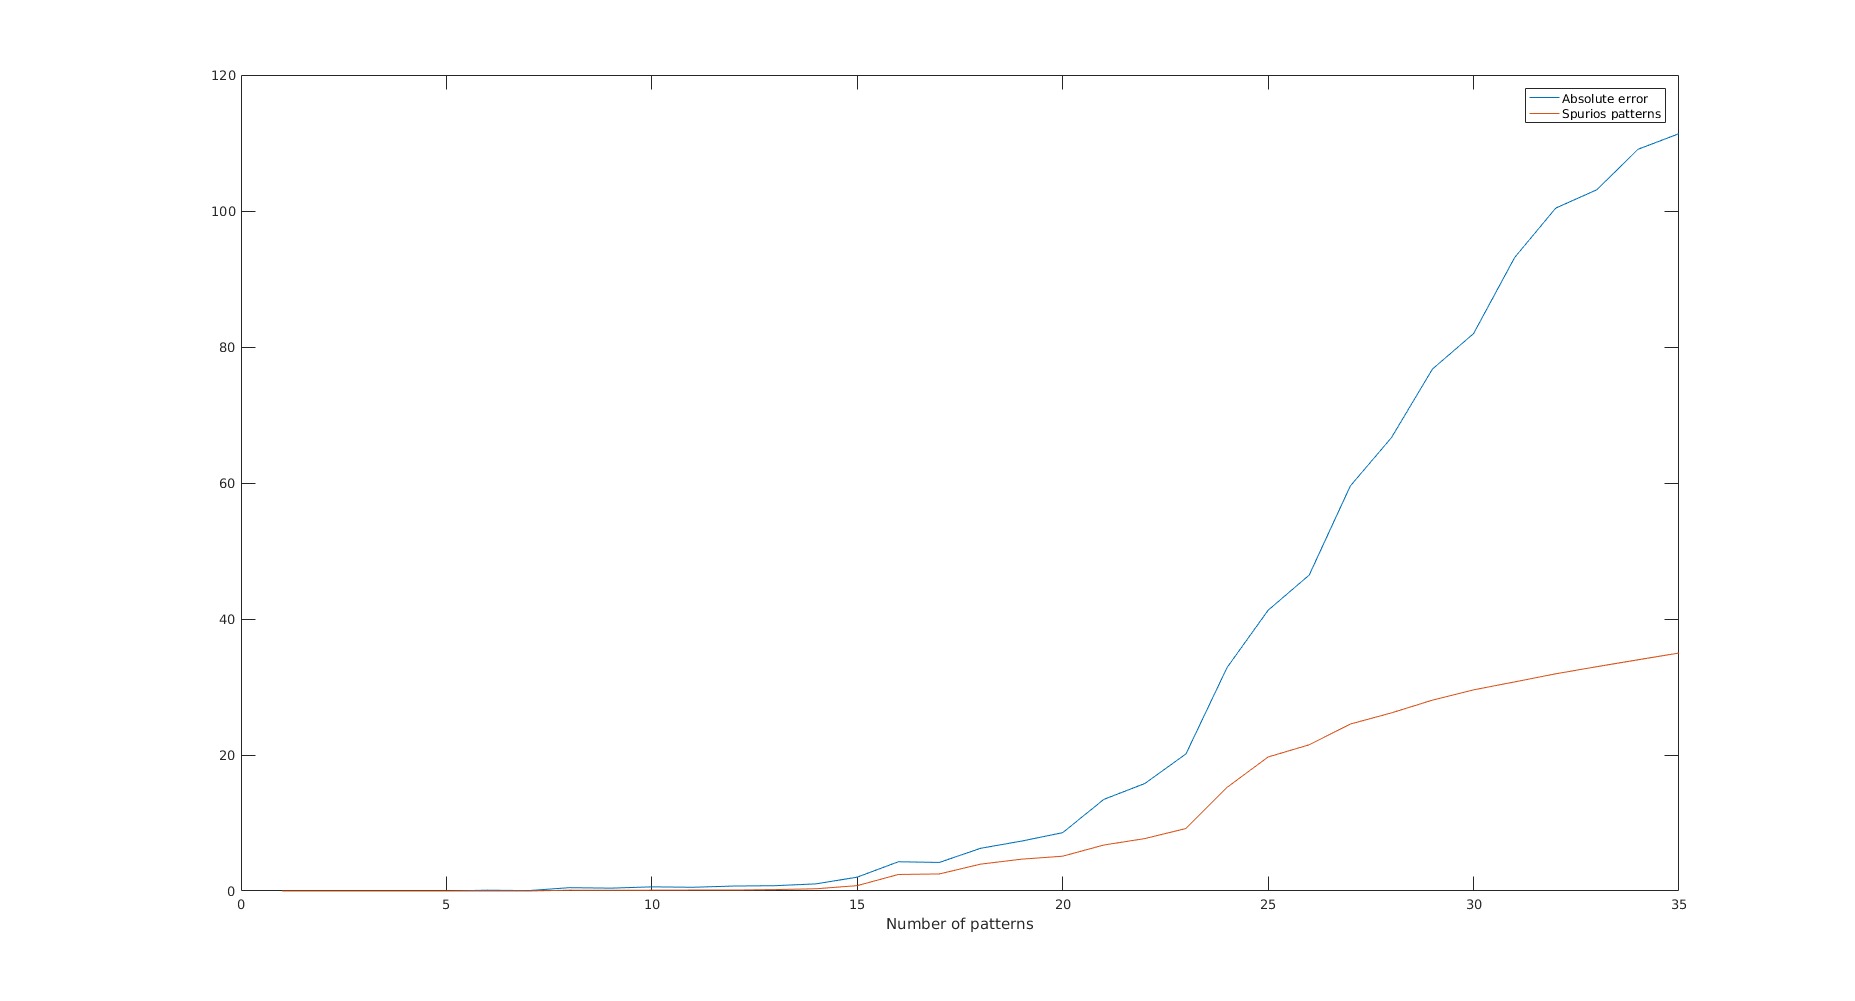
\includegraphics[width=\textwidth/2]{final/spurious_error_state}
\centering
\end{figure}

\begin{figure}[!htbp]
\caption{Theoretical loading capacity using the Hebb-rule.}
\label{teoretical_hebb}
\medbreak
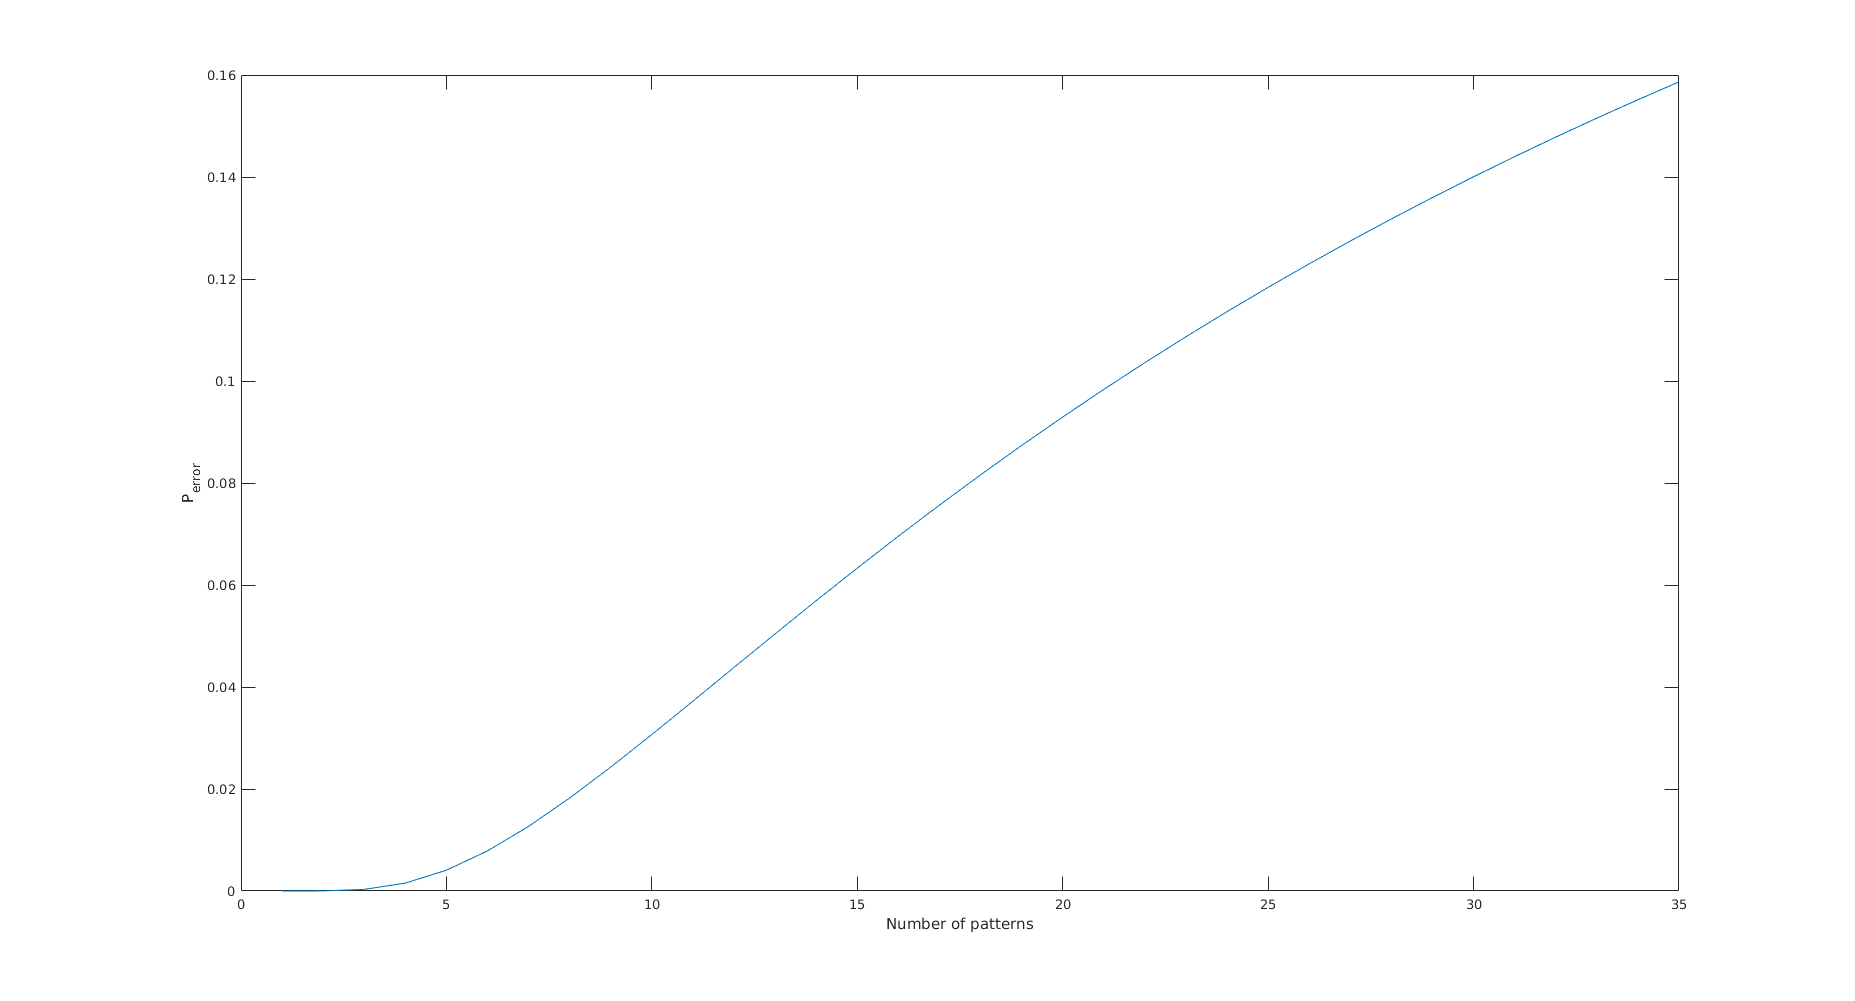
\includegraphics[width=\textwidth/2]{final/teoretical_hebb}
\centering
\end{figure}
\bigbreak
An alternative to overcome this downside of the Hopfield network can be a powerful, yet simple, FFNN. In fact, a FFNN was implemented with one hidden layer  using the default settings and 10 neurons in the hidden layer and 35 neurons in the output layer. A dataset of 1,000 samples was created. 80\% of samples were used as training test and validation test and the rest was used as test set. The overall CCR of the FFNN was 96.71\%. Figure \ref{neural_network_35_ouputs} shows the results of the first 5 predictions.

\begin{figure}[!htbp]
\caption{Top: Original letter. Middle: distorted letter by 3 pixeles. Bottom: prediction of the FFNN.}
\label{neural_network_35_ouputs}
\medbreak
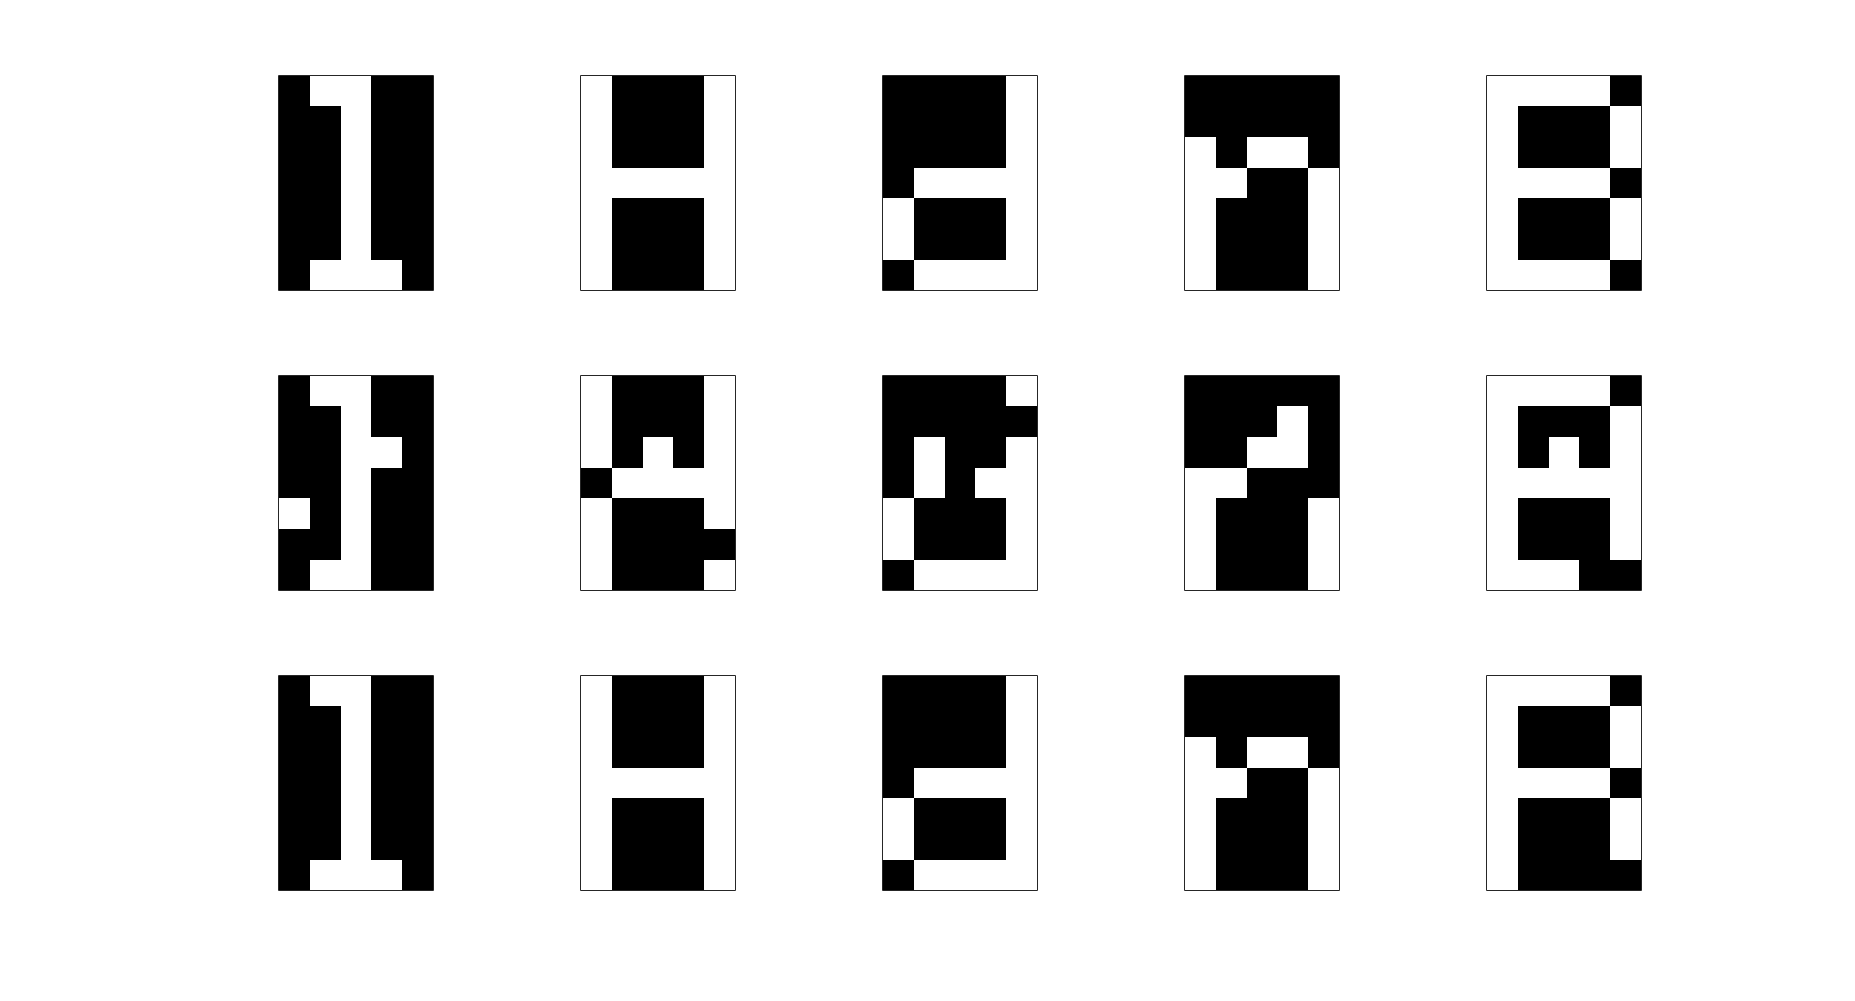
\includegraphics[width=\textwidth/2]{final/neural_network_35_ouputs}
\centering
\end{figure}
